\chapter{Phương pháp tiếp cận}
\noindent Ở phần này, phương pháp tiếp cận tính được sử dụng trong khóa luận sẽ được trình bày -- bằng cách sử dụng học tự giám sát, ta có thể để giải quyết phần nào vấn đề mà hệ thống gợi ý còn gặp phải. Ở phần trước, ta đã biết khái niệm về Học tự giám sát (Self-supervised Learning), về mạng học sâu đồ thị (Graph Neural Network). Phần này, ta sẽ tập trung tìm hiểu sự liên quan giữa dữ liệu tương tác người dùng -- sản phẩm và dạng biểu diễn đồ thị của dữ liệu đó. Tăng cường dữ liệu (Data Augmentation) đã được trình bày, tuy nhiên chỉ mới đề cập đến hiệu quả của nó trên hình ảnh, ngôn ngữ. Khi áp dụng trên dữ liệu đồ thị, cách thức, hiệu quả của nó mang lại cũng sẽ được trình bày cụ thể hơn, từ đó cho thấy việc áp dụng trên dạng dữ liệu đặc biệt này có gì khác so với dữ liệu dạng hình ảnh, văn bản,.... Sau đó, ta sẽ thảo luận về việc áp dụng Học tự giám sát vào hệ thống gợi ý như thế nào, mang lại hiệu quả như thế nào so với các phương pháp tiếp cận trước.
% 1. Cách áp dụng ssl trên gcn: cách áp dụng data augmentation trên graph --> cách áp dụng self supervised learning (contrastive learning) trên graph
% 2. SSR: có gì khác so vs học sâu graph bth? ssl task loss?? main task loss?? <--> Collaborative filtering + neighborhood aggregation (GCN)??
% 3. Phân tích model

\section{Tăng cường dữ liệu đồ thị} \label{3.1-data-aug}

\noindent Chúng ta đã biết các mô hình học sâu hiện nay luôn trong tình trạng `đói dữ liệu'. Ta càng cung cấp cho mô hình học càng nhiều dữ liệu, chất lượng đầu ra của mô hình có thể càng cải thiện. Nếu thiếu dữ liệu mô hình sẽ thiếu tính tổng quát hóa hoặc có thể dễ bị overfitting. Vậy nên ta rút ra được, có vẻ càng nhiều dữ liệu thì càng tốt, đây sẽ là lúc ta cần áp dụng phương pháp tăng cường dữ liệu nhằm tăng hiệu quả của việc học biểu diễn. Ở phần này, ta sẽ mô tả cụ thể việc tăng cường dữ liệu được áp dụng như thế nào trên dữ liệu dạng đồ thị. Sau khi có được dữ liệu tăng cường, ta sẽ sử dụng chúng ra sao.

Ở chương trước, ta đã biết về kỹ thuật tăng cường dữ liệu (data augmentation) và ứng dụng của nó trên các bài toán Thị giác máy tính (CV) hay Xử lý ngôn ngữ tự nhiên (NLP). Khi áp dụng vào hệ thống gợi ý, ta cần thay đổi về cách thức nhưng nhìn chung về ý tưởng cốt lõi vẫn sẽ giống nhau. Áp dụng cùng cách thức tương tự như trên các bài toán CV hay NLP là bất khả thi \cite{SGL} cho dữ liệu dạng đồ thị vì một vài lí do. Thứ nhất, các đặc trưng của người dùng và sản phẩm là rời rạc, vậy nên các tăng cường trên ảnh như là ngẫu nhiên crop, xoay, hay làm mờ không thể áp dụng được. Thứ hai, data trong CV và NLP là cô lập, trong khi người dùng và sản phẩm trong đồ thị tương tác là có kết nối với nhau và phụ thuộc lẫn nhau.

Khi áp dụng tăng cường dữ liệu, một số cách chọn thay đổi cấu trúc đồ thị, một số khác vẫn giữ nguyên cấu trúc của đồ thị, thay vì đó sẽ xáo trộn nhỏ các đặc trưng của node khiến nó trở nên bất biến với các thuộc tính ban đầu của node \cite{survey:aug-for-dgl, survey:ssl-for-rec-sys}.

% \subsection{Tăng cường cấu trúc đồ thị} \label{3.1.1-graph-structure-aug}
Ở phần này, ta sẽ mô tả các phương pháp phổ biến để tăng cường cấu trúc của đồ thị ban đầu, tức là tăng cường tập node $V$ và tập cạnh $E$. Hiệu quả của nó đã được chứng minh thông qua các model GMAE \cite{GMAE}, MGAE \cite{MGAE}, GraphCL \cite{GraphCL}. Một số phương pháp thường được sử dụng có thể liệt kê như dưới đây.

\begin{itemize}
    \item[] \textbf{Edge/Node Dropout}: với phần trăm tỉ lệ số cạnh muốn xóa/giữ lại, ta có thể  bỏ đi ngẫu nhiên một số cạnh hoặc một số node và các cạnh liên kết với chúng của đồ thị hiện tại nhằm tạo ra các đồ thị mới, bên cạnh đó cũng muốn giữ cấu trúc cơ bản của đồ thị. Ý tưởng này bắt nguồn từ việc chỉ một phần cạnh/node mới đóng góp hữu ích vào việc học biểu diễn và bỏ đi một số kết nối thừa thãi giúp biểu diễn của đồ thị ít bị ảnh hưởng bởi nhiễu. Biểu diễn toán học của đồ thị tăng cường với dropout như sau:
    \vspace*{-8mm}
    \begin{figure}[H]
        \null\hfill
        % 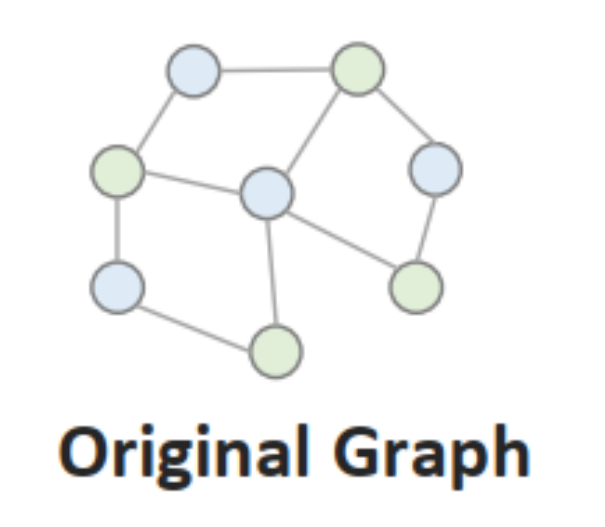
\includegraphics[scale=0.15]{images/Chapter3/original_graph.png}\\
        \begin{subfigure}{0.41\textwidth}
            % \centering
            % 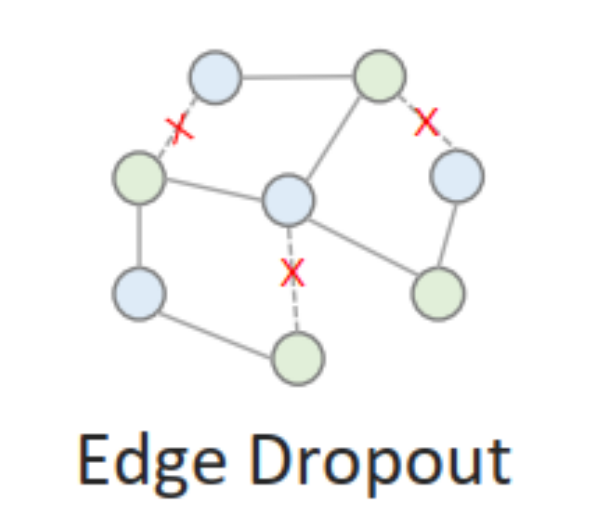
\includegraphics[scale=0.15]{images/Chapter3/edge_dropout.png}
            % \vspace*{-3mm}
            \[
            G_{\text{ED}} = (V, \mathbf{M}_{\text{ED}} \odot E),
            \]
            \caption{Edge dropout augmentation}
        \end{subfigure}
        % \hspace*{+5mm}
        \begin{subfigure}{0.41\textwidth}
            % \centering
            % 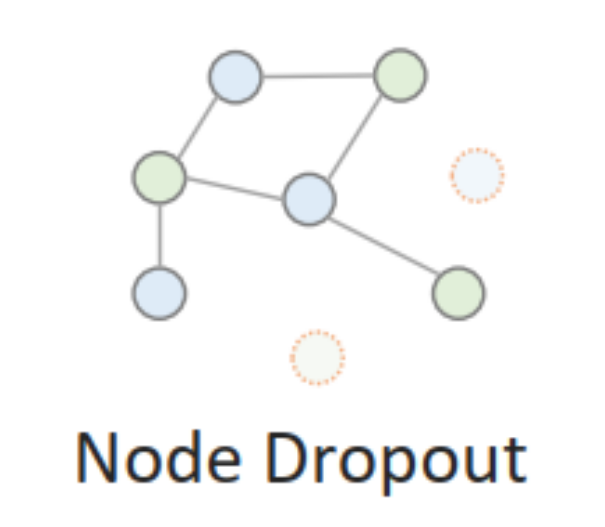
\includegraphics[scale=0.15]{images/Chapter3/node_dropout.png}
            % \vspace*{-3mm}
            \[
            G_{\text{ND}} = (\mathbf{M}_{\text{ND}} \odot V, \mathbf{M}_{\text{ND}}' \odot E),
            \]
            \caption{Node dropout augmentation}
        \end{subfigure}
        \hspace*{+15mm}
        \begin{subfigure}{0\textwidth}
            \begin{equation}\end{equation}
            \vspace*{+7.5mm}
        \end{subfigure}
    \end{figure}
    trong đó, $\mathbf{M}_{\text{ED}} \in \{0, 1\}^{|E|}$ là một masking vector để giúp sinh ra đồ thị tăng cường mà đã bỏ đi một số cạnh; $\mathbf{M}_{\text{ND}} \in \{0, 1\}^{|V|}$ và $\mathbf{M'}_{\text{ND}} \in \{0, 1\}^{|E|}$ là 2 masking vector để sinh ra đồ thị đã được bỏ đi một số node và các cạnh liên kết với các node đó.
    
    \item[] \textbf{Graph Diffusion}: còn được gọi là \textit{Graph rewiring} \cite{graphs-curvature}, phương pháp này tạo ra augmentation dựa trên đặc trưng cấu trúc toàn cục của đồ thị. Cụ thể hơn là \textit{Graph diffusion} thêm cạnh giữa các node có liên kết gián tiếp với nhau thông qua các trọng số đã được tính trước. Biểu diễn toán học của tăng cường diffusion như sau:
    % \begin{center}
    %     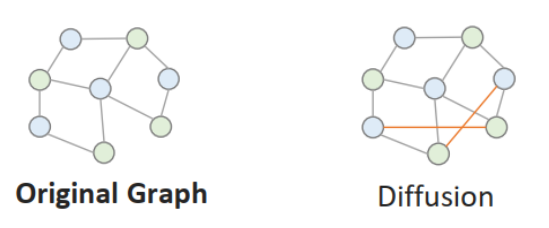
\includegraphics[scale=0.4]{images/Chapter3/graph_diffusion.png}
    % \end{center}
    % \vspace*{-\baselineskip}
    \begin{equation}
        G_{\text{Diff}} = (V, E \cup \tilde{E}),
    \end{equation}
    trong đó $\tilde{E}$ là tập cạnh được thêm vào.

    \item[] \textbf{Node Insertion}: chèn node cũng là một cách thường được sử dụng nhằm mục đích cải thiện Message passing hoặc các liên kết trên đồ thị gốc. Kỹ thuật này thêm các node ảo và các cạnh giữa các node ảo tới các node ban đầu. Biểu diễn toán học của phương pháp tăng cường này như sau:
    \begin{equation}
        G_{\text{NI}} = (V \cup \tilde{V}, E \cup \tilde{E}),
    \end{equation}
    trong đó $\tilde{V}$ và $\tilde{E}$ lần lượt là tập node được thêm và tập cạnh nối giữa $\tilde{V}$ và $V$.

    \item[] \textbf{Subgraph Sampling}: lấy mẫu ngẫu nhiên đồ thị con dựa vào một phần các node và cạnh liên kết của chúng từ đồ thị ban đầu. Phương pháp này khá giống Edge/Node dropout, nhưng thay vì lấy mẫu một cách ngẫu nhiên, đồ thị con mà phương pháp này cho ra thỏa mãn một số tính chất nào đó. Thông thường là sẽ lấy mẫu đồ thị con nhỏ mà bảo tồn càng nhiều thông tin cho việc học càng tốt \cite{data-aug-for-GNN, GNN-via-topo-denoising}. Một lợi thế của phương pháp này là giúp bảo toàn cấu trúc cục bộ trong đồ thị. Biểu diễn toán học của phương pháp tăng cường là:
    % \begin{center}
    %     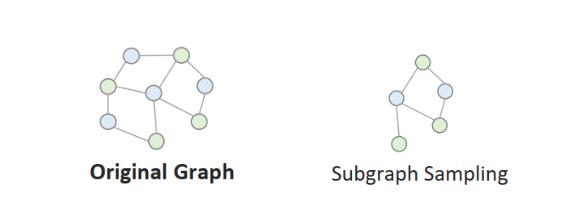
\includegraphics[scale=0.55]{images/Chapter3/subgraph_sampling.png}
    % \end{center}
    % \vspace*{-\baselineskip}
    \begin{equation}
        G_{\text{Sampled}} = (\bm{\mathcal{F}}(V), \bm{\mathcal{F'}}(E)),
    \end{equation}
    trong đó, $\bm{\mathcal{F}}(\cdot)$ và $\bm{\mathcal{F'}}(\cdot)$ lần lượt là hàm lấy mẫu cho các node và cạnh.\\
    Một trong những biến thể phổ biến của Subgraph sampling được áp dụng là \textit{Random walk} \cite{GCC}, từ đồ thị gốc ta chọn một tập node bất kỳ, từ đó lần lượt đi qua các node kề một cách ngẫu nhiên cho đến khi đạt đến số lượng node cần được đi qua cho trước hoặc một đặc tính nào đó đã được thỏa mãn. Nói cách khác là với mỗi node trong tập, ta lấy ra một đồ thị con chứa node đó và các node đã được ``đi qua'', rồi hợp nhất các đồ thị con đó lại.
    \begin{equation}
        G_{RW} = (\mathbf{M}_{RW} \odot V, \mathbf{M}_{RW}' \odot E),
    \end{equation}
    với $\mathbf{M}_{RW}$ là masking vector trích các node đã được chọn và các node được đi qua sau random walk, $\mathbf{M'}_{RW}$ là masking vector trích các cạnh được đi qua.
\end{itemize}


% \subsection{Tăng cường đặc trưng đồ thị}

% \noindent Khác với cách tiếp cận cấu trúc đồ thị, lần này ta sẽ tập trung biến đổi ma trận đặc trưng $\mathbf{X}$. Các phương pháp áp dụng theo hướng tăng cường đặc trưng đồ thị cũng khá phổ biến như các model MGM \cite{MGM}, BGRL \cite{BGRL}.

% \begin{itemize}
%     \item[] \textbf{Feature Corruption}: với phương pháp này, ta sẽ thêm nhiễu vào các đặc trưng của node ban đầu \cite{graph-adversarial-training} hoặc thêm vào biểu diễn đặc trưng đã học \cite{graph-adversarial-SSL}. Biểu diễn toán học của phương pháp corruption này như sau:
%     \[
%     \tilde{x}_i = x_i + c_i,
%     \]
%     trong đó $x_i$ là vector đặc trưng ban đầu hoặc đã học của node $i$, $c_i$ là vector nhiễu.

%     \item[] \textbf{Feature Shuffling}: phương pháp này thay đổi thông tin ngữ cảnh bằng cách đổi hàng và cột trong ma trận đặc trưng $\mathbf{X}$. Biểu diễn toán học là:
%     \[
%     \mathbf{X}_{\text{FS}} = \mathbf{P}_r \mathbf{X} \mathbf{P}_c,
%     \]
%     trong đó, $\mathbf{P}_r \in \{0, 1\}^{n \times n}$ và $\mathbf{P}_c \in \{0, 1\}^{d \times d}$ là ma trận hoán vị cột và dòng, trong 2 ma trận này, mỗi dòng và mỗi cột chỉ chứa duy nhất một giá trị bằng 1.

%     \item[] \textbf{Feature Masking}: bằng cách “che lại” thuộc tính của vài node bằng các mask (một mask được tạo bằng cách lấy sample từ một phân phối chuẩn). Nói dễ hiểu hơn ta sẽ khiến một phần đặc trưng node bằng 0 với một xác suất nào đó. Biểu diễn toán học như sau:
%     \[
%     \mathbf{X}_{\text{FM}} = \mathbf{X} \odot \mathbf{M},
%     \]
%     trong đó $\mathbf{M}$ là ma trận masking với $\mathbf{M}_{ij} = 0$ nếu đặc trưng $j$ của node $i$ bị lược bỏ, $\mathbf{M}_{ij} = 1$ nếu ngược lại.

%     \item[] \textbf{Feature Mixing:} trộn các đặc trưng của node này với các đặc trưng của node khác để tạo ra một node mới. Biểu diễn toán học của việc trộn này như sau:
%     \[
%     \tilde{x} = \alpha x_i + (1 - \alpha) x_j,
%     \]
%     trong đó $\alpha \in [0, 1]$ là hệ số trộn biểu diễn tỉ lệ lấy thông tin giữa $x_i$ và $x_j$.
    
% \end{itemize}

\section{Học trên đồ thị cho hệ thống gợi ý} \label{3.2-graph-learning-recommender}
% 3.2. Học trên đồ thị cho hệ thống gợi ý
% 1. Đồ thị tương tác
% 2. BPR loss
% 3. LightGCN
\subsection{Đồ thị tương tác}
\noindent Để tiện cho phần này, ngoài biểu diễn đồ thị $G$ theo tập node $V$ và cạnh $E$, ta còn có thể biểu diễn nó theo một ma trận kề $\mathbf{A} \in \mathbb{R}^{|V| \times |V|}$ với các giá trị $a_{uv}$ bằng 1 hoặc bằng 0 thể hiện việc có tồn tại cạnh nối giữa hai node $u$ và $v$ hay không. Tức là $\forall u, v \in V, a_{uv} = 1 \Leftrightarrow (u, v) \in E$.

Đối với thông tin phản hồi thu thập được của người dùng, ta có thể chia ra làm 2 loại \cite{CF-for-implicit-feedback} là \textit{Explicit feedback -- phản hồi tường minh} (đánh giá điểm một sản phẩm, viết review, like/dislike...) và \textit{Implicit feedback -- phản hồi ngầm} (click vào trang sản phẩm, hành động mua sản phẩm...). Có thể thấy rằng phản hồi tường minh có lợi thế rất lớn đó là thông tin phản hồi được cung cấp rõ ràng minh bạch, cụ thể hơn, và cho model nhiều thông tin ngữ cảnh hơn; trong khi phản hồi ngầm thì không rành mạch, và không phản ánh đánh giá thực sự của người dùng đối với sản phẩm. Tuy nhiên hầu hết dữ liệu phản hồi của người dùng đối với sản phẩm lại là phản hồi ngầm \cite{denoise-implicit-feedback} vì nhiều lí do như đa số người dùng miễn cưỡng về việc để lại đánh giá/viết review, trong nhiều trường hợp thì việc thu thập dữ liệu tường minh lại còn rất tốn kém về thời gian, tiền bạc và công sức. Cần phải nói thêm là lượng dữ liệu phản hồi này thường là rất lớn, đặc biệt là về lĩnh vực thương mại điện tử \cite{large-scale-amazon-reviews}, do đó, ta sẽ tập trung vào khai thác tập dữ liệu phản hồi ngầm của người dùng, và cũng bỏ qua các mối quan hệ/tương tác giữa người dùng và người dùng, sản phẩm và sản phẩm, cùng với các thuộc tính ban đầu mà các đối tượng đó có thể có (tuổi, giới tính...; loại sản phẩm, kích thước...).

Ta có thể coi dữ liệu phản hồi này như là một đồ thị liên kết giữa người dùng với sản phẩm mà họ đã tương tác, trong đó mỗi node đại diện cho một thực thể người dùng hoặc sản phẩm, và cạnh giữa 2 node người dùng và sản phẩm tồn tại nếu và chỉ nếu người dùng đó đã tương tác với sản phẩm đó. Cụ thể hơn, giả sử ta có tập dữ liệu người dùng $U$ và sản phẩm $I$, cùng với lịch sử tương tác của họ, ta rút ra được đồ thị $G = (V, E)$ mà $V = U \cup I$ là các node và $E = \{(u, i) | u \in U, i \in I\}$ là các cạnh với 2 node $u$, $i$ có tương tác. Lấy ví dụ hình \ref{subfig:interaction-graph}, với $U = \{u_0, u_1, u_2, u_3\}$ và $I = \{i_0, i_1, i_2, i_3, i_4\}$.

\begin{figure}[H]
    \centering
    \begin{subfigure}[b]{0.3\textwidth}
        \centering
        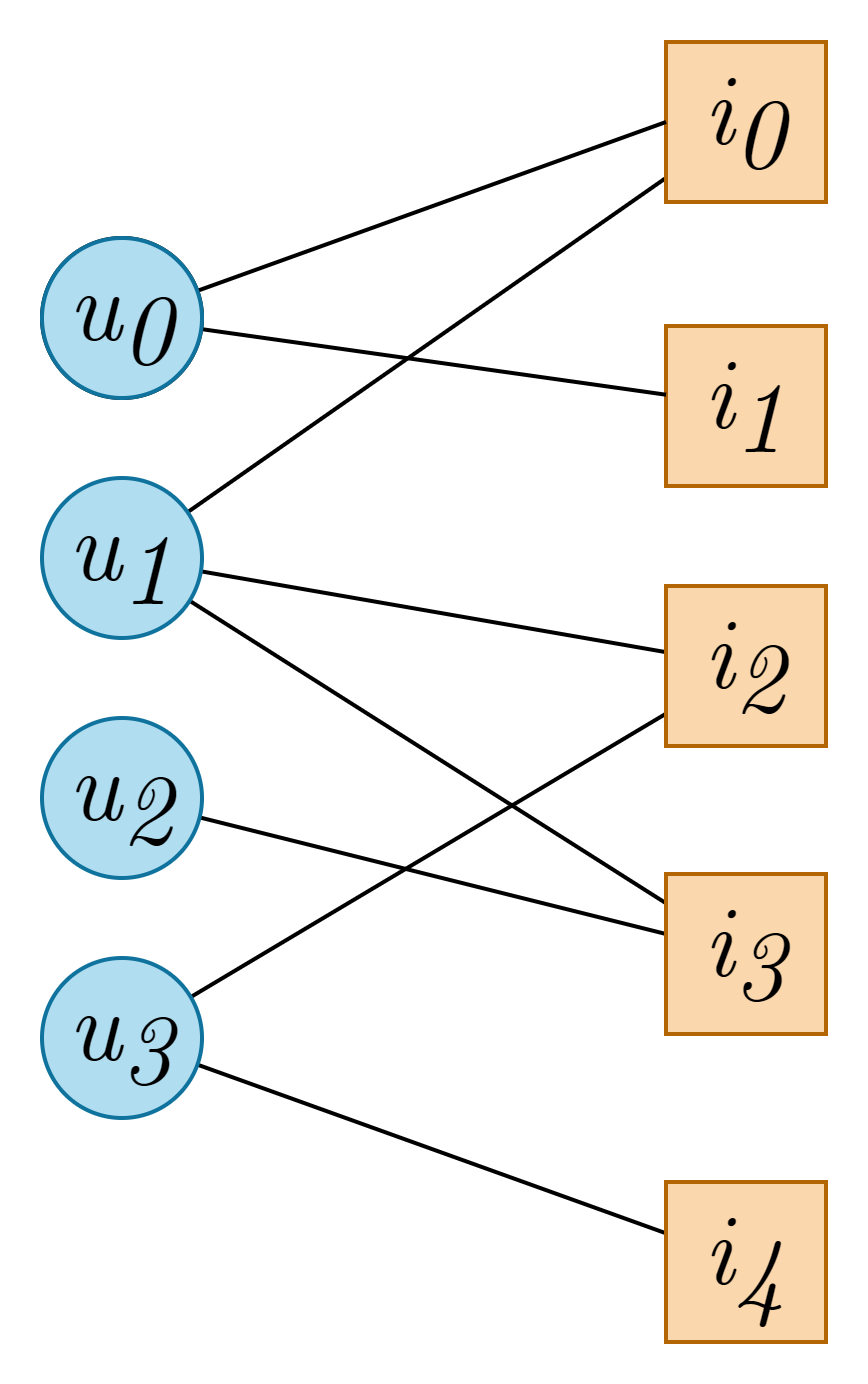
\includegraphics[scale=0.13]{images/Chapter3/user-item_graph.png}
        \subcaption{Đồ thị tương tác.}
        \label{subfig:interaction-graph}
    \end{subfigure}
    \begin{subfigure}[c]{0.12\textwidth}
        \centering
        \vspace*{-65mm}
        \LARGE$\Longleftrightarrow$
    \end{subfigure}
    \begin{subfigure}[b]{0.4\textwidth}
        \centering
        \resizebox{\columnwidth}{!} {
            \centering
            \renewcommand{\arraystretch}{1.2}
            \begin{tabular}{ccc|c|c|c|c|}
                \multicolumn{1}{c}{} & & \multicolumn{5}{c}{Sản phẩm} \\
                \multicolumn{1}{c}{} & \multicolumn{1}{c||}{} &\multicolumn{1}{r|}{$i_0$} & $i_1$ & $i_2$ & $i_3$ & $i_4$ \\
                \hhline{~=::=====}
                \multirow{4}*{\rotatebox[origin=c]{90}{Người dùng}}  
                & \multicolumn{1}{c||}{$u_0$} & \multicolumn{1}{r|}{1} & 1 & 0 & 0 & 0 \\
                \hhline{~-||-----}
                & \multicolumn{1}{c||}{$u_1$} & \multicolumn{1}{r|}{1} & 0 & 1 & 1 & 0 \\
                \hhline{~-||-----}
                & \multicolumn{1}{c||}{$u_2$} & \multicolumn{1}{r|}{0} & 0 & 0 & 1 & 0 \\
                \hhline{~-||-----}
                & \multicolumn{1}{c||}{$u_3$} & \multicolumn{1}{r|}{0} & 0 & 1 & 0 & 1 \\
                \hhline{~-||-----}
            \end{tabular}
        }
        \vspace*{10mm}
        \subcaption{Ma trận tương tác.}
        \label{subfig:interaction-matrix}
    \end{subfigure}
    \caption[Đồ thị và ma trận tương tác.]{Đồ thị tương tác (trái) và ma trận tương tác (phải) giữa người dùng và sản phẩm.}
\end{figure}

\noindent Để biểu diễn dữ liệu đồ thị trên máy tính, ta có thể dùng một ma trận tương tác (hình \ref{subfig:interaction-matrix}) $\mathbf{R} \in \mathbb{R}^{|U|\times|I|}$ trong đó $r_{ui} = 1$ nếu $(u, i) \in E$ và $r_{ui} = 0$ nếu ngược lại. Cuối cùng, một ma trận kề tổng quát của đồ thị có thể được xây dựng như sau:
\begin{equation}
    \mathbf{A} = \begin{pmatrix}
        \mathbf{0} & \mathbf{R} \\
        \mathbf{R}^T & \mathbf{0}
    \end{pmatrix}
    \label{adj-mat-from-R}
\end{equation}

Các giá trị trong ma trận $\mathbf{R}$ đại diện cho lịch sử tương tác và không nhất thiết phải là 0 hoặc 1, một số lớn hơn có thể đại diện cho tần số tương tác và cũng có thể là ngữ cảnh thêm cho hệ thống gợi ý. Để đơn giản hóa, ta sẽ chỉ quan tâm tới việc có tương tác hay không giữa các đối tượng mà không xét đến tần suất tương tác.

Cũng có thể nhận ra là đồ thị tương tác là một đồ thị hai phía -- \textit{Bipartite graph} \cite{bipartite-graph-partition}, đó là đồ thị mà có thể chia tập node $V$ ra làm 2 tập (ví dụ $U$ và $I$) mà không có cạnh nối bất kỳ 2 node nào trong cùng một tập, và có một số đặc điểm có ích cho tác vụ recommendation. Vì đồ thị này được tạo ra từ các tương tác người dùng với sản phẩm nên sẽ chứa tín hiệu Collaborative filtering \cite{MGAT}. Cụ thể là láng giềng liền kề (lịch sử tương tác với sản phẩm đối với node người dùng; hoặc tập các người dùng đã tương tác đối với node sản phẩm) chính là mô tả của node đó và có thể xem là đặc trưng của node. Láng giềng ở bước nhảy thứ 2 mô tả những người dùng/sản phẩm tương tự.
% Với tính chất của dữ liệu tương tác, ta có thể nói ma trận kề $\mathbf{A}$ và ma trận đặc trưng $\mathbf{X}$ của đồ thị tương tác (đã nhắc đến ở đầu phần \ref{3.1.1-graph-structure-aug}) là một.

\subsection{Bayesian Personalized Ranking loss}
\noindent \textbf{Bayesian Personalized Ranking (BPR)} \cite{BPR-loss} là một phương pháp để tối ưu hóa tham số của một model gợi ý dự đoán ranking (đánh giá) của người dùng về một sản phẩm dựa trên dữ liệu tương tác ngầm của người dùng.

Ta sẽ phân tích kỹ ma trận tương tác $\mathbf{R}$. Nhắc lại, $r_{ui} = 1$ có nghĩa là có tương tác giữa người dùng $u$ và sản phẩm $i$, giả sử là tương tác ``người dùng mua sản phẩm'', $r_{ui} = 0$ có nghĩa là không có tương tác. Điểm đặc biệt của phản hồi ngầm là khi có tương tác giữa người dùng và sản phẩm thì có khả năng rất cao là, và sẽ được coi như là, tương tác ``tích cực'' \cite{BPR-loss} (người dùng thích sản phẩm, đánh giá cao...). Đáng lẽ là khi thu thập dữ liệu thì ta có thêm một giá trị âm cho $r_{ui}$ để đại diện cho tương tác ``tiêu cực'' (người dùng không thích sản phẩm). Tuy nhiên trong thực tế thì những tương tác tiêu cực đó hầu như không có. Một giải thích đơn giản là khi người dùng mua sản phẩm thì thường là họ đã biết trước họ sẽ mua cái gì rồi. Những cặp người dùng -- sản phẩm không có tương tác thì một là do người dùng thực sự không thích sản phẩm, hai là dữ liệu bị thiếu/không rõ ràng (họ đang để dành tiền, họ chưa bao giờ thấy sản phẩm đó nhưng có khả năng sẽ thích nó...). Như vậy giá trị ma trận \ref{subfig:interaction-matrix} có thể hiểu như ma trận \ref{subfig:raw-data} ở ví dụ sau:

\begin{figure}[H]
    \centering
    \begin{subfigure}[c]{0.4\textwidth}
        \centering
        \resizebox{\columnwidth}{!} {
            \centering
            \renewcommand{\arraystretch}{1.2}
            \begin{tabular}{cc|c|c|c|c|}
                \multicolumn{1}{c||}{} &\multicolumn{1}{r|}{$i_0$} & $i_1$ & $i_2$ & $i_3$ & $i_4$ \\
                \hhline{=::=====}
                \multicolumn{1}{c||}{$u_0$} & \multicolumn{1}{r|}{+} & + & \textcolor{orange}{\textbf{?}} & \textcolor{orange}{\textbf{?}} & \textcolor{orange}{\textbf{?}} \\
                \hhline{-||-----}
                \multicolumn{1}{c||}{$u_1$} & \multicolumn{1}{r|}{+} & \textcolor{orange}{\textbf{?}} & + & + & \textcolor{orange}{\textbf{?}} \\
                \hhline{-||-----}
                \multicolumn{1}{c||}{$u_2$} & \multicolumn{1}{r|}{\textcolor{orange}{\textbf{?}}} & \textcolor{orange}{\textbf{?}} & \textcolor{orange}{\textbf{?}} & + & \textcolor{orange}{\textbf{?}} \\
                \hhline{-||-----}
                \multicolumn{1}{c||}{$u_3$} & \multicolumn{1}{r|}{\textcolor{orange}{\textbf{?}}} & \textcolor{orange}{\textbf{?}} & + & \textcolor{orange}{\textbf{?}} & + \\
                \hhline{-||-----}
            \end{tabular}
        }
        \subcaption{Dữ liệu mà $\mathbf{R}$ diễn tả.}
        \label{subfig:raw-data}
    \end{subfigure}
    \begin{subfigure}[c]{0.15\textwidth}
        \centering
        \Large$\dashrightarrow$
    \end{subfigure}
    \begin{subfigure}[c]{0.4\textwidth}
        \centering
        \resizebox{\columnwidth}{!} {
            \centering
            \renewcommand{\arraystretch}{1.2}
            \begin{tabular}{cc|c|c|c|c|}
                \multicolumn{1}{c||}{} &\multicolumn{1}{r|}{$i_0$} & $i_1$ & $i_2$ & $i_3$ & $i_4$ \\
                \hhline{=::=====}
                \multicolumn{1}{c||}{$u_0$} & \multicolumn{1}{r|}{+} & + & \textcolor{orange}{+} & \textcolor{orange}{+} & \textcolor{orange}{--} \\
                \hhline{-||-----}
                \multicolumn{1}{c||}{$u_1$} & \multicolumn{1}{r|}{+} & \textcolor{orange}{--} & + & + & \textcolor{orange}{+} \\
                \hhline{-||-----}
                \multicolumn{1}{c||}{$u_2$} & \multicolumn{1}{r|}{\textcolor{orange}{--}} & \textcolor{orange}{--} & \textcolor{orange}{+} & + & \textcolor{orange}{--} \\
                \hhline{-||-----}
                \multicolumn{1}{c||}{$u_3$} & \multicolumn{1}{r|}{\textcolor{orange}{+}} & \textcolor{orange}{--} & + & \textcolor{orange}{--} & + \\
                \hhline{-||-----}
            \end{tabular}
        }
        \subcaption{Dữ liệu tương tác có thể có.}
    \end{subfigure}
    \caption[Dữ liệu diễn tả tương tác ngầm.]{Dữ liệu diễn tả tương tác ngầm và thiếu (trái), và dữ liệu có thể có (phải).}
    \label{subfig:interpreted-matrix}
\end{figure}

\noindent trong đó, dấu $+$ biểu diễn tương tác tích cực, $-$ biểu diễn tương tác tiêu cực, và \textcolor{orange}{\textbf{?}} là giá trị thiếu.

Tuy là dữ liệu có giá trị thiếu và ma trận $\mathbf{R}$ chỉ biểu diễn tương tác, ta sẽ coi việc ``người dùng $u$ tương tác với sản phẩm $i$ mà không có tương tác với sản phẩm $j$'' đồng nghĩa với việc ``$u$ ưa thích $i$ hơn $j$'', tức là $r_{ui} = 1$ và $r_{uj} = 0$. Ngoài ra, những cặp sản phẩm $(i, j)$ mà $r_{ui} = r_{uj}$ ngụ ý là mức độ ưa thích của $u$ với $i$ và $j$ là như nhau hoặc không thể kết luận được. Xét cho cùng thì dự đoán một giá trị tương tác tích cực hay một giá trị tiêu cực là rất khó nếu dữ liệu tương tác có dạng như trên. Thay vì đó, ta sẽ dự đoán xem người dùng sẽ xếp thứ hạng (rank) những sản phẩm trong tập sản phẩm như thế nào.

Rendle và các cộng sự \cite{BPR-loss} định nghĩa một quan hệ toán học $>_u \in I^2$ mang ý nghĩa so sánh mức độ yêu thích của người dùng trên tập sản phẩm $I$. Đó là khi ta nói \(i >_u j\; (i, j \in I)\) thì có nghĩa là người dùng $u$ thích sản phẩm $i$ hơn sản phẩm $j$. Quan hệ này mang tính chất thứ tự toàn phần, cụ thể:
\begin{align*}
    & \forall i, j \in I: i \neq j \implies i >_u j \lor j >_u i \tag{toàn phần} \\
    & \forall i, j \in I: i >_u j \land j >_u i \implies i = j \tag{phi đối xứng} \\
    & \forall i, j, k \in I: i >_u j \land j >_u k \implies i >_u k \tag{bắc cầu}
\end{align*}
Để tiện hơn, ta cũng định nghĩa:
\begin{equation}
    \begin{aligned}
        I_u^+ & = \{i \in I \; | \; (u, i) \in E\}, \\
        U_i^+ & = \{u \in U \; | \; (u, i) \in E\}, \\
        D & = \{(u, i, j) \; | \; i \in I_u^+ \land j \in I \setminus I_u^+\},
    \end{aligned}
\end{equation}
trong đó, $I_u^+$ là tập các sản phẩm mà người dùng $u$ tương tác, $U_i^+$ là tập các người dùng có tương tác với sản phẩm $i$, $D$ là tập các bộ ba $(u, i, j)$ đại diện cho người dùng $u$ thích sản phẩm $i$ hơn $j$. Ngoài ra, $D$ còn sẽ đại diện cho dữ liệu huấn luyện. Rendle và công sự đưa ra 2 ưu điểm \cite{BPR-loss} của cách tiếp cận này:
\begin{itemize}
    \item[1.] Dữ liệu huấn luyện bao gồm các tương tác tích cực, tiêu cực và dữ liệu bị thiếu. Hai sản phẩm thiếu dữ liệu tương tác của người dùng sẽ là hai sản phẩm mà ta cần phải dự đoán cái nào được đánh thứ hạng cao hơn. Vì vậy, xét theo cặp sản phẩm thì tập huấn luyện $D$ và tập test thử nghiệm là rời nhau.

    \item[2.] Dữ liệu huấn luyện có duy nhất một mục đích là để giúp huấn luyện dự đoán ranking.
\end{itemize}

Giả sử ta có tập tham số $\Theta$ (một vector nhiều chiều) của một model gợi ý bất kỳ. Để tìm đúng ranking cá nhân cho các sản phẩm, công thức BPR nhắm tìm giá trị cho $\Theta$ để tối đại hóa xác suất hậu nghiệm sau:
\begin{equation}
    p(\Theta | >_u) \propto p(>_u | \Theta) p(\Theta),
\end{equation}
kí hiệu $>_u$ ở đây là cấu trúc của sự ưa thích đối với người dùng $u$, nói cách khác, kí hiệu đại diện cho ranking cá nhân mong muốn của người dùng $u$ trên tập sản phẩm.

Ta có hai giả định đối với dữ liệu: (i) thứ tự các cặp sản phẩm $(i, j)$ trong quan hệ ưa thích của mỗi người dùng là độc lập với nhau, và (ii) tất cả người dùng hành động độc lập với nhau. Từ giả định (i), ta có thể viết lại hàm likelihood $p(>_u | \Theta)$ cho người dùng $u$ bằng cách triển khai tích xác suất như sau:
\begin{equation}
    p(>_u | \Theta) = \prod_{(i,j) \in I \times I}{p(i >_u j | \Theta)^{\delta((u,i,j) \in D)} \cdot \left(1 - p(i >_u j | \Theta)\right)^{\delta((u,j,i) \notin D)}},
\end{equation}
với $\delta(b)$ bằng 1 nếu mệnh đề $b$ đúng, bằng 0 nếu ngược lại. Giả định (ii) cho thấy rằng xác suất $p$ có thể được kết hợp với tất cả $u \in U$. Cùng với (i), ta có:
\begin{equation}
    \prod_{u \in U}{p(>_u | \Theta)} = \prod_{(u,i,j) \in U \times I \times I}{p(i >_u j | \Theta)^{\delta((u,i,j) \in D)} \cdot \left(1 - p(i >_u j | \Theta)\right)^{\delta((u,j,i) \notin D)}}
    \label{eq:prod-p}
\end{equation}
Nhờ vào tính toàn phần và phi đối xứng, công thức trên có thể được đơn giản hóa như sau:
\begin{equation}
    \prod_{u \in U}{p(>_u | \Theta)} = \prod_{(u,i,j) \in D}{p(i >_u j | \Theta)}
\end{equation}
Tuy nhiên, tới đây vẫn chưa thể lập một thứ tự ranking cho một người dùng được. Để đảm bảo cả 3 tính chất toàn phần, phi đối xứng và bắc cầu của quan hệ $>_u$, Rendle \cite{BPR-loss} định nghĩa xác suất người dùng ưa thích sản phẩm $i$ hơn $j$ như sau:
\begin{equation}
    p(i >_u j | \Theta) = \sigma(\hat{x}_{uij}(\Theta)),
\end{equation}
với $\sigma(x)$ là hàm logistic sigmoid:
\begin{equation}
    \sigma(x) = \frac{1}{1 + e^{-x}}
\end{equation}
Hàm $\hat{x}_{uij}(\Theta)$ là một hàm số thực nhận $\Theta$ là đầu vào, và nắm bắt được mối quan hệ giữa người dùng $u$, sản phẩm $i$ và $j$. Nói cách khác, $\hat{x}_{uij}$ phải thể hiện được mức độ ưa thích của $u$ với $i$ như thế nào so với $j$. Để tiện hơn, ta sẽ bỏ qua tham số $\Theta$ khi viết $\hat{x}_{uij}$ cho các công thức ở sau.

Để hoàn thiện hướng tiếp cận, ta xem $p(\Theta)$ như là phân phối chuẩn với mean bằng 0 và ma trận variance-covariance $\Sigma_{\Theta}$:
\begin{equation}
    p(\Theta) \sim \mathcal{N}(0, \Sigma_{\Theta})
\end{equation}
Để giảm số lượng hyperparameter, ta đặt $\Sigma_{\Theta} = \lambda_{\Theta} \mathbf{I}$, với $\mathbf{I}$ là ma trận đơn vị cùng kích thước với $\Sigma_{\Theta}$. Bài toán tối ưu sẽ quy về tìm cực đại của:
\begin{equation}
    \begin{aligned}
        \text{BPR-Opt} & = \ln{p(\Theta | >_u)} \\
                       & = \ln{(p(>_u | \Theta) p(\Theta))} \\
                       & = \ln{\left(\prod_{(u,i,j) \in D}{\sigma(\hat{x}_{uij})} p(\Theta)\right)} \\
                       & = \sum_{(u,i,j) \in D}{\ln{\sigma(\hat{x}_{uij})}} + \ln{p(\Theta)} \\
                       & = \sum_{(u,i,j) \in D}{\ln{\sigma(\hat{x}_{uij})}} - \lambda_{\Theta} \lVert \Theta \rVert^2,
    \end{aligned}
    \label{eq:bpr-opt}
\end{equation}
trong đó, $\lambda_{\Theta}$ là tham số regularization của model. Vì $i$ được xem như là ``ưa thích hơn'' $j$ đối với $u$, ta có thể chọn một công thức sao cho $\hat{x}_{uij}$ phản ánh được điều đó. Như vậy, ta có thể đơn giản hóa $\hat{x}_{uij}$ như sau:
\begin{equation}
    \hat{x}_{uij} = \hat{y}_{ui} - \hat{y}_{uj},
    \label{eq:xuij-as-yuij}
\end{equation}
trong đó, $\hat{y}_{ui}$ và $\hat{y}_{uj}$ lần lượt là ranking dự đoán của người dùng $u$ đối với $i$ và $j$. Cơ bản là công thức trên cho biết sự khác nhau giữa dự đoán về độ ưa thích với hai sản phẩm $i$ và $j$. Theo công thức \eqref{eq:bpr-opt} và ngữ cảnh là cực đại hóa BPR-Opt, công thức thay thế cho $\hat{x}_{uij}$ ở trên cũng tương tự như là việc ``thúc đẩy'' ranking của $i$ sao cho cao hơn $j$ cho người dùng $u$.

Từ \eqref{eq:bpr-opt} và \eqref{eq:xuij-as-yuij}, ta có hàm mất mát sau cho một model gợi ý:
\begin{equation}
    \begin{aligned}
        \mathcal{L}_{\text{BPR}} & = -\text{BPR-Opt} \\
                                 & = -\sum_{(u,i,j) \in D}{\ln{\sigma(\hat{y}_{ui} - \hat{y}_{uj})}} + \lambda_{\Theta} \lVert \Theta \rVert^2
    \end{aligned}
    \label{eq:bpr-loss}
\end{equation}

\subsection{Áp dụng học đồ thị lên hệ thống gợi ý} \label{3.2.3-GNN-on-rec}

\noindent Về việc học trên đồ thị cho tác vụ gợi ý thì đã tồn tại một số model \cite{PinSAGE, GC-MC, NGCF, LightGCN} được sử dụng khá phổ biến. Trong PinSAGE \cite{PinSAGE}, Ying và các cộng sự xây dựng một framework baseline, học biểu diễn để giúp tăng chất lượng học cho một thuật toán học downstream gợi ý khác; GC-MC \cite{GC-MC} và NGCF \cite{NGCF} là hai trong những model đầu tiên áp dụng học trên đồ thị để khai tác tín hiệu collaborative filtering. Trong khóa luận này, \textbf{LightGCN} \cite{LightGCN}, một model nhẹ và hiệu quả, sẽ được chọn cho việc học và dự đoán gợi ý trên đồ thị tương tác. Cũng cần phải nhắc đến là hướng tiếp cận học đồ thị trong phạm vi khóa luận này là một thuật toán học đặc biệt mà trong đó toàn bộ dữ liệu, cùng với nhau, có cấu trúc/phân phối/đặc trưng của một đồ thị và có nhiệm vụ dự đoán các tính chất của đồ thị hoặc một phần đồ thị đó (\textit{transductive learning}) \cite{GCN-model, DGCN, NGCF}, tức là model không thể đưa ra dự đoán cho bộ dữ liệu với cấu trúc đồ thị khác \cite{review:GNN}. Trái với một loại khác của học đồ thị mà trong đó mỗi mẫu dữ liệu là một đồ thị riêng và model đưa ra dự đoán trên dữ liệu chưa từng thấy (\textit{inductive learning}) \cite{GraphSAGE, PinSAGE, GC-model, GG-NN}. Tuy nhiên khi áp dụng học đồ thị thì ý tưởng và cách học của 2 loại model này là tương tự nhau.

\subsubsection{Mô tả LightGCN}

\noindent Các công trình ứng dụng học mạng tích chập đồ thị cho hệ thống gợi ý trước khi LightGCN ra đời thiếu sự phân tích kỹ lưỡng về cách giảm độ phức tạp của mạng tích chập đồ thị để phù hợp hơn với tác vụ gợi ý, trong khi mạng tích chập đồ thị lại được tạo ra để giải quyết một phạm vi lớn các vấn đề liên quan đến đồ thị và có rất nhiều phép tính trong mạng neuron. Theo tìm hiểu của các tác giả của LightGCN, Xiangnan He và các đồng nghiệp \cite{LightGCN}, hai trong những đặc điểm phổ biến của một mạng học máy đồ thị là biến đổi đặc trưng -- \textit{feature transformation}, và hàm kích hoạt phi tuyến tính -- \textit{nonlinear activation} không những không có tác động đáng kể đến việc khai thác tín hiệu collaborative filtering, mà còn tăng độ phức tạp cho việc huấn luyện và làm giảm chất lượng của dự đoán. Mục tiêu của LightGCN là đơn giản hóa thiết kế chung của mạng tích chập đồ thị, giúp mô hình nhẹ hơn và phù hợp hơn với tác vụ gợi ý.

\subsubsection{Thiết kế tích chập của LightGCN}
\noindent Ta đã đề cập đến kiến trúc chung của mạng học đồ thị ở phần \ref{2.2.3-GNN-design}. Gọi $\mathbf{e}_u^{(l)}$ và $\mathbf{e}_i^{(l)}$ lần lượt là các embedding của người dùng $u$ và sản phẩm $i$ tại lớp thứ $l$; gọi $\mathcal{N}_u$ là tập sản phẩm mà người dùng $u$ tương tác, và $\mathcal{N}_i$ là tập các người dùng có tương tác với sản phẩm $i$. Tác vụ tích chập (Neighborhood aggregation) của LightGCN được định nghĩa như sau:
\begin{equation}
    \begin{aligned}
        \mathbf{e}_u^{(l+1)} & = \sum_{i \in \mathcal{N}_u}{\frac{1}{\sqrt{|\mathcal{N}_u|} \sqrt{|\mathcal{N}_i|}} \mathbf{e}_i^{(l)}}, \\
        \mathbf{e}_i^{(l+1)} & = \sum_{u \in \mathcal{N}_i}{\frac{1}{\sqrt{|\mathcal{N}_i|} \sqrt{|\mathcal{N}_u|}} \mathbf{e}_u^{(l)}},
    \end{aligned}
    \label{lightgcn-neiagg}
\end{equation}
với hệ số bình thường hóa $\frac{1}{\sqrt{|\mathcal{N}_u|} \sqrt{|\mathcal{N}_i|}}$ được lấy từ thiết kế của model GCN \cite{GCN-model}, mục đích của hệ số là làm giảm sự gia tăng nhanh chóng của các giá trị trong vector embedding khi chạy quá trình tích chập qua nhiều lớp. Có một số công thức khác có thể thay thế cho hệ số này, nhưng các tác giả của LightGCN tìm hiểu thấy là cách làm này cũng đủ tốt. Hàm tích chập được chọn của LightGCN chỉ là một hàm tổng có trọng số đơn giản, hoàn toàn không có biến đổi đặc trưng hay kích hoạt phi tuyến gì cả, giúp model nhẹ hơn nhiều.

Để ý kỹ là với mỗi node $u$ hoặc $i$, ta không tổng hợp embedding của chính node đó từ lớp trước mà chỉ tổng hợp các node láng giềng. Lý do là tác vụ tổng hợp các embedding lại để sử dụng cho tác vụ dự đoán (sẽ nói trong phần tiếp theo) có thể nắm bắt việc tổng hợp chính các node đó rồi.

\subsubsection{Kết hợp các embedding cho dự đoán}
\noindent Trong model LightGCN, các tham số học $\Theta$ của model chính là embedding ban đầu của các node, tức là embedding tại lớp thứ 0, $\{\mathbf{e}_u^{(0)} | u \in U\}$ và $\{\mathbf{e}_i^{(0)} | i \in I\}$; các embedding lớp thứ 0 có thể được lấy ngẫu nhiên từ một phân phối nào đó. Sau khi tích chập được $L$ lớp, các embedding cuối cùng của các node sẽ được kết hợp như sau:
\begin{equation}
    \mathbf{e}_u = \sum_{l=0}^{L}{\alpha_l \mathbf{e}_u^{(l)}}, \qquad
    \mathbf{e}_i = \sum_{l=0}^{L}{\alpha_l \mathbf{e}_i^{(l)}},
\end{equation}
trong đó, $\alpha_l \geq 0$ định nghĩa mức độ quan trọng (trọng số) của lớp thứ $l$ và có thể được coi như là hyperparameter hoặc là tham số cho một mạng attention \cite{survey:attention-models, attentive-CF}. Theo thử nghiệm của He và đồng nghiệp \cite{LightGCN}, đặt các giá trị $\alpha_l$ đều bằng $1/(K+1)$ cũng đủ để giúp model đạt hiệu suất tốt, một lý do khác là để giữ tính đơn giản và nhẹ của model.

\noindent Các tác giả của LightGCN đưa ra 3 lý do \cite{LightGCN} tại sao lại chọn tổng hợp các embedding như thế này để đưa vào tác vụ dự đoán:
\begin{itemize}
    \item[(1)] Khi số lớp trong model càng nhiều thì các embedding sẽ chịu nhiều ảnh hưởng của vấn đề ``làm nhẵn'' -- oversmoothing \cite{insights-GCN}, tức là các embedding sẽ bị kéo lại gần nhau, các embedding ở các cụm khác nhau càng trở nên khó phân biệt. Vậy nên nếu chỉ sử dụng lớp cuối cùng để đưa ra dự đoán là rất rắc rối.

    \item[(2)] Các embedding ở mỗi lớp nắm bắt những đặc điểm khác nhau. Ví dụ embedding ở lớp thứ nhất chứa thông tin về những người dùng và sản phẩm có tương tác, embedding ở lớp thứ hai chứa nắm bắt thông tin về những người dùng, sản phẩm tương tự nhau, và các embedding ở lớp cao hơn nắm bắt những đặc điểm bậc cao \cite{NGCF}. Việc kết hợp các embedding ở nhiều lớp sẽ giúp biểu diễn của node toàn diện hơn.

    \item[(3)] Như đã nói ở trước, kết hợp embedding của node ở tất cả các lớp giúp cho việc tổng hợp chính node đó mà không cần phải thể hiện qua tác vụ tích chập.
\end{itemize}

\noindent Cuối cùng, ta có kết quả dự đoán ranking $\hat{y}_{ui}$ của người dùng $u$ với sản phẩm $i$ là tích vô hướng của embedding của $u$ và $i$:
\begin{equation}
    \hat{y}_{ui} = \mathbf{e}_u^T \mathbf{e}_i,
\end{equation}

\noindent Và ta có biểu đồ thể hiện thiết kế của LightGCN như sau:
\begin{figure}[H]
    \centering
    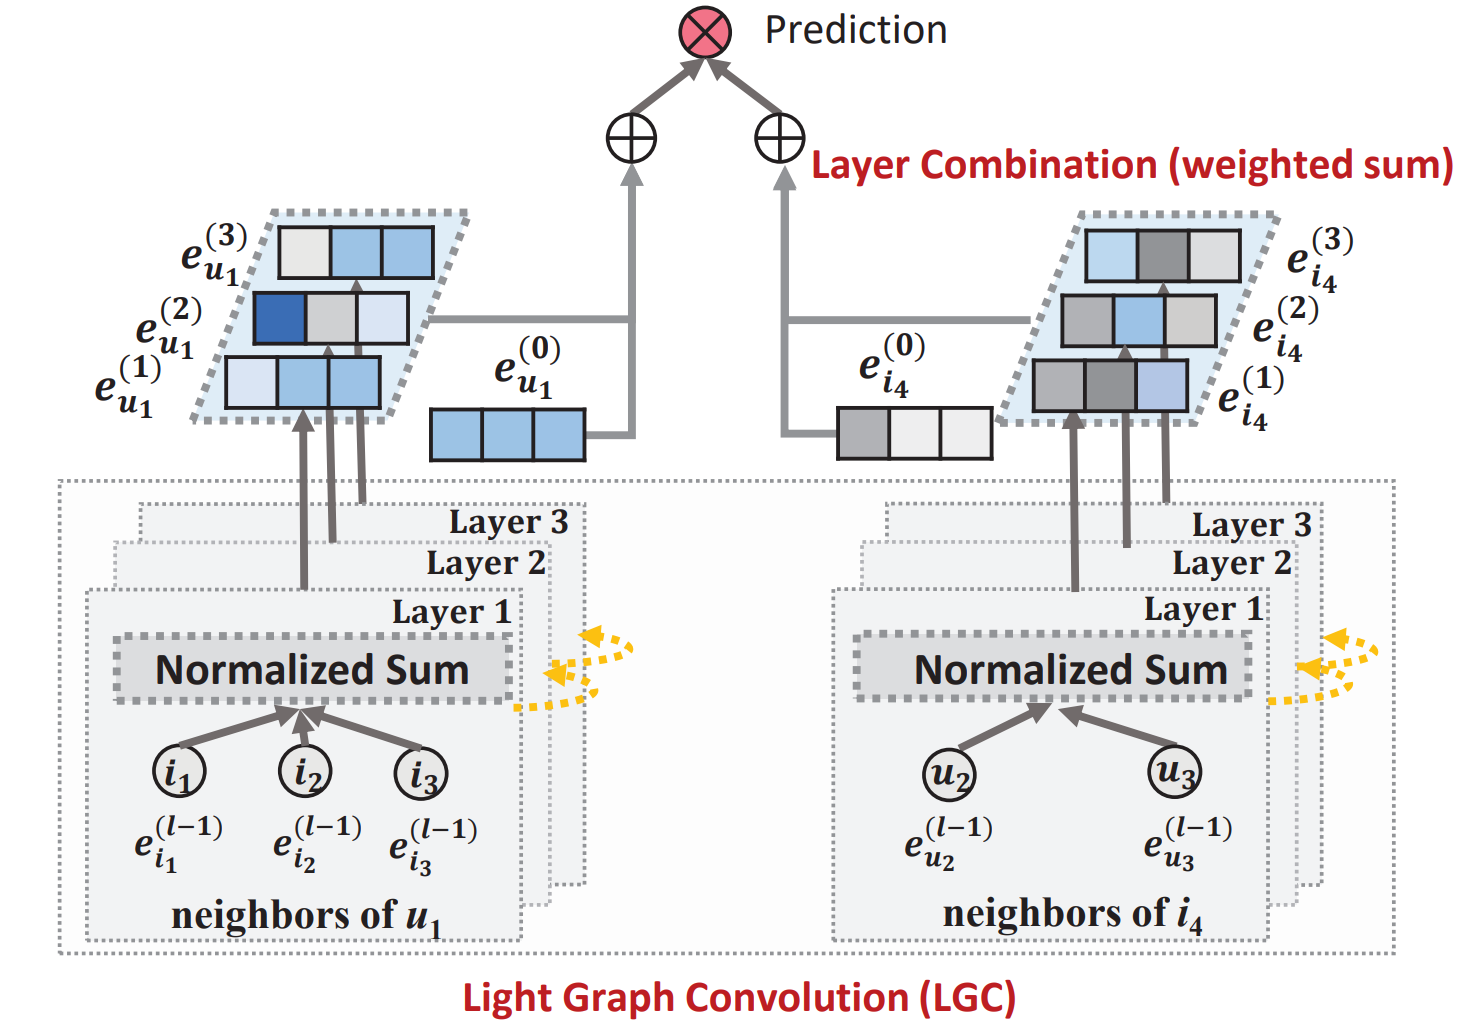
\includegraphics[scale=0.35]{images/Chapter3/lightgcn.png}
    \caption{Thiết kế của LightGCN.}
\end{figure}

\subsubsection{Biểu diễn ma trận của các phép toán}
\noindent Để tiện tính toán trên máy, các tác giả của LightGCN lập ra các phép toán tích chập dưới dạng ma trận. Đầu tiên, ta có ma trận tương tác $\mathbf{R} \in \mathbb{R}^{|U|\times|I|}$, như công thức \eqref{adj-mat-from-R}, ta có ma trận kề:
\begin{equation}
    \mathbf{A} = \begin{pmatrix}
        \mathbf{0} & \mathbf{R} \\
        \mathbf{R}^T & \mathbf{0}
    \end{pmatrix},
\end{equation}
Với các giá trị ban đầu của embedding (lớp 0), ta lập ma trận $\mathbf{E}^{(0)} \in \mathbb{R}^{(|U| + |I|) \times d}$ với $d$ là số chiều embedding, dòng thứ $i$ của $\mathbf{E}^{(0)}$ là $\mathbf{e}_i^{(0)}$. Ta có dạng ma trận của công thức \eqref{lightgcn-neiagg} là:
\begin{equation}
    \mathbf{E}^{(l+1)} = (\mathbf{D}^{-\frac{1}{2}} \mathbf{A} \mathbf{D}^{-\frac{1}{2}}) \mathbf{E}^{(l)},
\end{equation}
trong đó, $\mathbf{D}$ là ma trận đường chéo, cho biết bậc của node trong đồ thị tương tác với kích thước $(|U| + |I|) \times (|U| + |I|)$, có nghĩa là giá trị $D_{ii}$ trong ma trận cho biết số lượng node láng giềng của $i$ trong đồ thị. Như vậy, embedding tổng hợp cuối cùng được định nghĩa là:
\begin{equation}
    \begin{aligned}
        \mathbf{E} & = \alpha_0 \mathbf{E}^{(0)} + \alpha_1 \mathbf{E}^{(1)} + \alpha_2 \mathbf{E}^{(2)} + ... + \alpha_L \mathbf{E}^{(L)} \\
                   & = \alpha_0 \mathbf{E}^{(0)} + \alpha_1 \tilde{\mathbf{A}} \mathbf{E}^{(0)} + \alpha_2 \tilde{\mathbf{A}}^2 \mathbf{E}^{(0)} + ... + \alpha_L \tilde{\mathbf{A}}^L \mathbf{E}^{(0)}
    \end{aligned}
    \label{eq:lightgcn-encoder}
\end{equation}
trong đó, $\tilde{\mathbf{A}} = \mathbf{D}^{-\frac{1}{2}} \mathbf{A} \mathbf{D}^{-\frac{1}{2}}$.


\section{Áp dụng mô hình Học Tự Giám Sát trên đồ thị tương tác người dùng -- sản phẩm}
\noindent Đã nhắc đến ở phần \ref{2.2.2-reprensentation-learning} và \ref{3.2-graph-learning-recommender}, việc học biểu diễn đã bước một bước tiến mới trong việc khai thác kết nối bậc cao hơn trong đồ thị người dùng -- sản phẩm. Tuy nhiên, ngoài những bất cập nói chung của hệ thống gợi ý nói chung (phần \ref{2.1.3-rec-issues}), việc kết hợp học trên đồ thị với gợi ý hiệu quả nhưng vẫn còn đang gặp một vài hạn chế \cite{SGL}.

\begin{itemize}
    \item[(1)] Tín hiệu học giám sát thưa thớt: vấn đề này cũng đã được đề cập. Phần lớn các model có thiết kế dạng học giám sát, tuy nhiên theo ta biết đối với tương tác người dùng với sản phẩm thì dữ liệu quan sát được là rất thưa so với toàn bộ không gian tương tác. Điều này khiến cho việc học biểu diễn không đạt hiệu quả như mong đợi.
    
    \item[(2)] Ảnh hưởng bởi nhiễu: vì hầu hết dữ liệu phản hồi của người dùng đối với sản phẩm lại là phản hồi ngầm thay vì là tường minh \cite{denoise-implicit-feedback} nên các tương tác quan sát được thường xuyên có chứa nhiễu bởi rất nhiều lý do, ví dụ người dùng bị lừa mua sản phẩm... Cơ chế tích chập của mạng tích chập đồ thị làm phóng đại ảnh hưởng của các tương tác lên việc học biểu diễn nên quá trình huấn luyện dễ bị ảnh hưởng do nhiễu trong tương tác.
    
    \item[(3)] Phân phối dữ liệu bị lệch: các tương tác quan sát được thường có phân phối lũy thừa \cite{power-law-dist}. Các sản phẩm bậc thấp thì thiếu tín hiệu giám sát, trong khi đó các sản phẩm có bậc cao thì lại xuất hiện thường xuyên hơn trong tác vụ Neighborhood aggregation và Supervised loss nên có ảnh hưởng nhiều hơn đến học biểu diễn.
\end{itemize}

Học tự giám sát mở ra một con đường mới cho việc giải quyết vấn đề dữ liệu thưa của bài toán hệ thống gợi ý. Mặc dù không có một định nghĩa rõ ràng nào về  việc áp dụng học tự giám sát lên hệ thống gợi ý (SSR), tuy nhiên ta có thể tóm tắt sơ qua về một số đặc điểm \cite{survey:ssl-for-rec-sys} cần lưu ý của SSR như sau:

\begin{itemize}
    \item[] \textbf{Thứ nhất}, mô hình thu được nhiều tín hiệu giám sát hơn bằng việc bán tự động khai thác chính dữ liệu thô ban đầu. Đây là ý tưởng cốt lõi của bất kỳ bài toán học tự giám sát nào từ trước đến nay.
    
    \item[] \textbf{Thứ hai}, ta sử dụng pretext task để train/pre-train mô hình gợi ý với dữ liệu tăng cường. Đây chính là điều khiến SSR khác với các phương pháp tiếp cận khác dùng để giải quyết bài toán hệ thống gợi ý hiện nay.
    
    \item[] \textbf{Thứ ba}, nhiệm vụ gợi ý đóng vai trò là nhiệm vụ chính, pretext task là nhiệm vụ phụ với vai trò tăng cường hiệu quả của nhiệm vụ gợi ý.
\end{itemize}

Hiện nay có rất nhiều phương thức tiếp cận SSR. Nhìn chung, mỗi model SSR chứa hai thành phần \cite{survey:ssl-for-rec-sys} chính: Encoder $\bm{f_\theta}$ và Projection head $\bm{g_\varphi}$. Encoder có thể là một mạng neuron (GNN, Multi-layer Perception...) với tập tham số học $\Theta$ và có nhiệm vụ học cách biểu diễn (embedding) $\mathbf{E}$ cho người dùng và sản phẩm từ dữ liệu. Projection head có cấu trúc đơn giản, có thể là một hàm tuyến tính, mapping, hoặc một mạng neuron đơn giản và có nhiệm vụ tối ưu hóa các biểu diễn đó cho nhiệm vụ gợi ý. Nói cách khác là bộ phận Head giúp model phân biệt tốt hơn những mẫu dữ liệu nào là giống nhau, những mẫu dữ liệu nào là khác nhau. Mạng SSR tập trung giải bài toán sau:
\begin{equation}
    f_\theta, g_\varphi, \mathbf{E} = \underset{f_\theta, g_\varphi}{arg min}\mathcal{L}\left(g_\varphi(f_\theta(\mathcal{D}, \tilde{\mathcal{D}}))\right),
\end{equation}
với $\mathcal{D}$ và $\tilde{\mathcal{D}}$ dữ liệu ban đầu và đã tăng cường, $\mathcal{L}$ là hàm mất mát kết hợp giữa tác vụ gợi ý $\mathcal{L}_\textit{rec}$ và tác vụ học không giám sát $\mathcal{L}_\textit{ssl}$. Từ tổng quát hóa trên, ta có thể phân thành 4 phương thức \cite{survey:ssl-for-rec-sys} SSR chủ yếu: \textbf{Contrastive Learning}, \textbf{Generative}, \textbf{Predictive} và \textbf{Hyrbrid}.
\begin{itemize}
    \item[] \textbf{Contrastive}: Kéo những bản sao tăng cường, gọi là các view, của cùng một instance (người dùng/sản phẩm) lại gần nhau, đẩy những view khác instance ra xa nhau trong không gian nhúng.\\
    \begin{minipage}{\linewidth}
        \vspace*{+5mm}
        \centering
        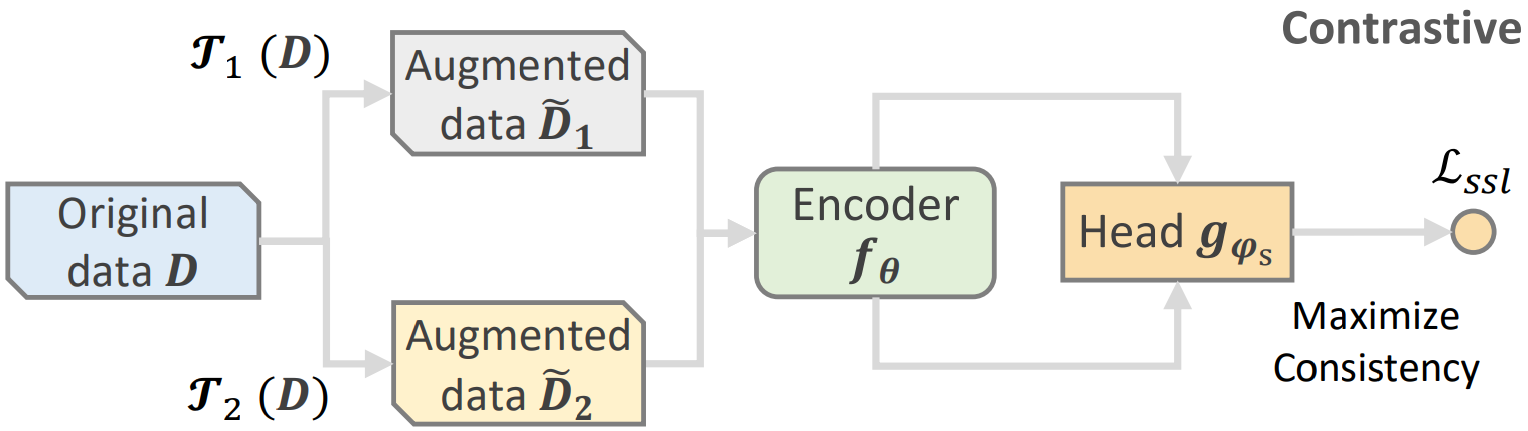
\includegraphics[scale=0.3]{images/Chapter3/contras_ssr.png}
        \captionof{figure}[Sơ đồ tổng thể phương pháp Contrastive trong bài toán Self-supervised Recommendation.]{Sơ đồ tổng thể phương pháp Contrastive trong bài toán Self-supervised Recommendation.}
    \end{minipage}
    
    \item[] \textbf{Generative}: Dự đoán một phần của data gốc ban đầu đã bị làm hỏng.\\
    \begin{minipage}{\linewidth}
        \vspace*{+5mm}
        \centering
        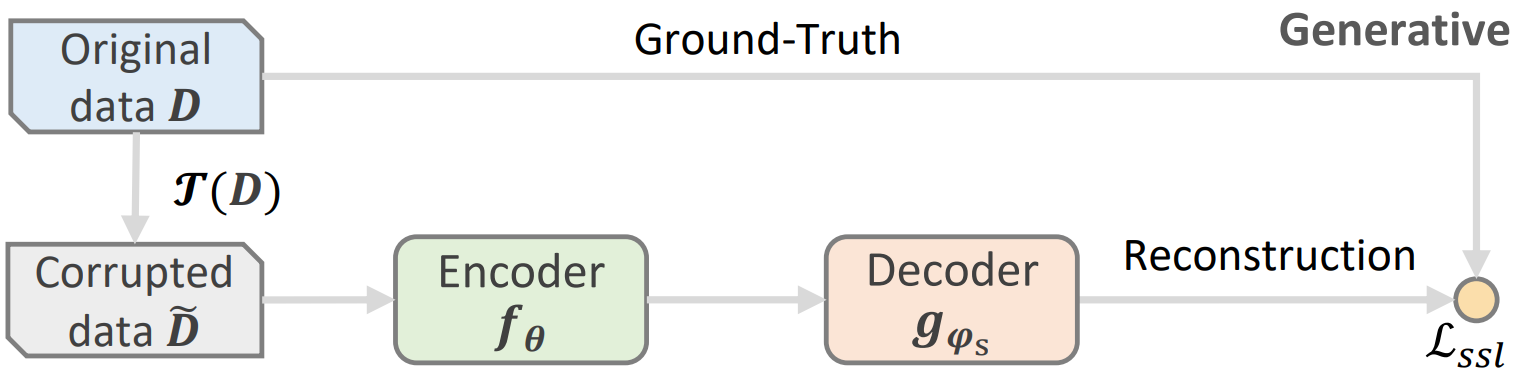
\includegraphics[scale=0.3]{images/Chapter3/gen_ssr.png}
        \captionof{figure}[Sơ đồ tổng thể phương pháp Generative trong bài toán Self-supervised Recommendation.]{Sơ đồ tổng thể phương pháp Generative trong bài toán Self-supervised Recommendation. Thành phần Decoder $\bm{g_\varphi}$ ở đây là một loại Head đặc biệt mà có nhiệm vụ tái tạo lại dữ liệu gốc từ dữ liệu embedding của dữ liệu đã bị làm hỏng. Sau đó dữ liệu này và dữ liệu gốc thực sự sẽ được so sánh với nhau.}
    \end{minipage}
    
    \item[] \textbf{Predictive}: Khá giống với phương pháp Generative. Nhưng trong khi mục tiêu của generative method là dự đoán data gốc, phương pháp Predictive, những mẫu dữ liệu mới hoặc nhãn dữ liệu mới sẽ được sinh ra để giúp tác vụ pretext.\\
    \begin{minipage}{\linewidth}
        \vspace*{+5mm}
        \centering
        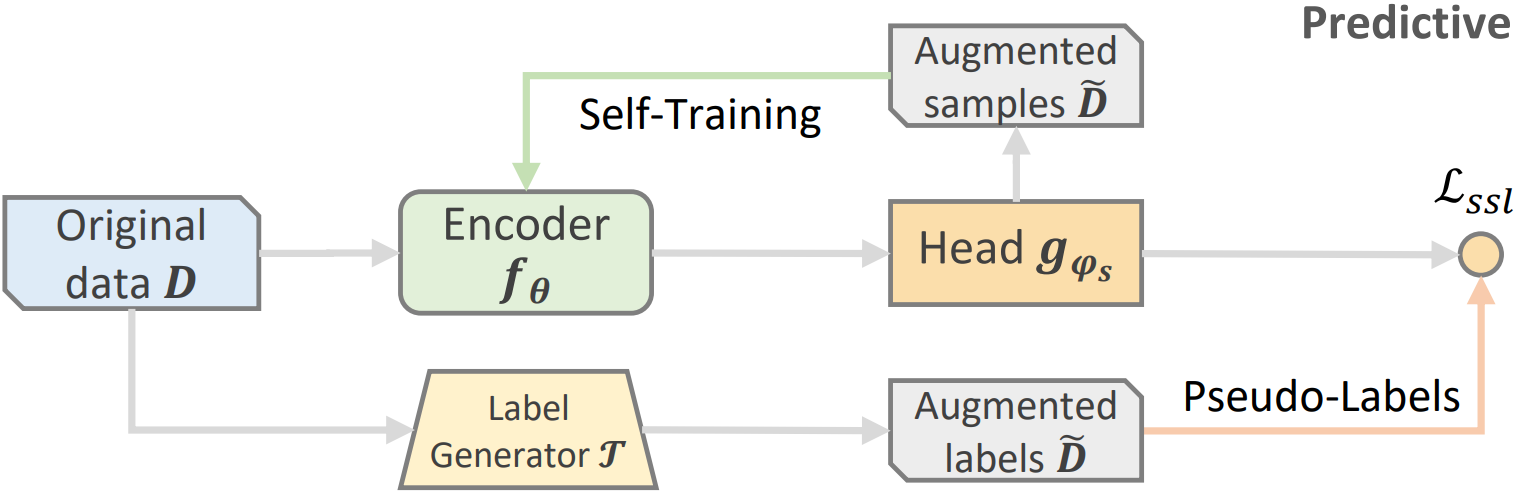
\includegraphics[scale=0.3]{images/Chapter3/pred_ssr.png}
        \captionof{figure}[Sơ đồ tổng thể phương pháp Predictive trong bài toán Self-supervised Recommendation.]{Sơ đồ tổng thể phương pháp Predictive trong bài toán Self-supervised Recommendation. Có thể chia phương pháp ra hai loại: dựa trên mẫu dữ liệu (sample-based) và dựa trên nhãn giả (pseudo-label-based). Loại thứ nhất tập trung dự đoán những mẫu dữ liệu nào là có thông tin hữu ích nhất cho pretext; loại thứ hai sinh ra nhãn giả cho dữ liệu dùng một Label Generator (có thể là một encoder khác) để giúp cho Encoder chính $\bm{f_\theta}$.}
    \end{minipage}
    
    \item[] \textbf{Hybrid}: Mỗi pretext task trên đều có ưu điểm riêng và đều có thể tận dụng được các self-supervision signal khác nhau. Hybrid method (phương pháp lai) tích hợp các pretext task khác nhau vào cùng một SSR model.\\
    \begin{minipage}{\linewidth}
        \vspace*{+5mm}
        \centering
        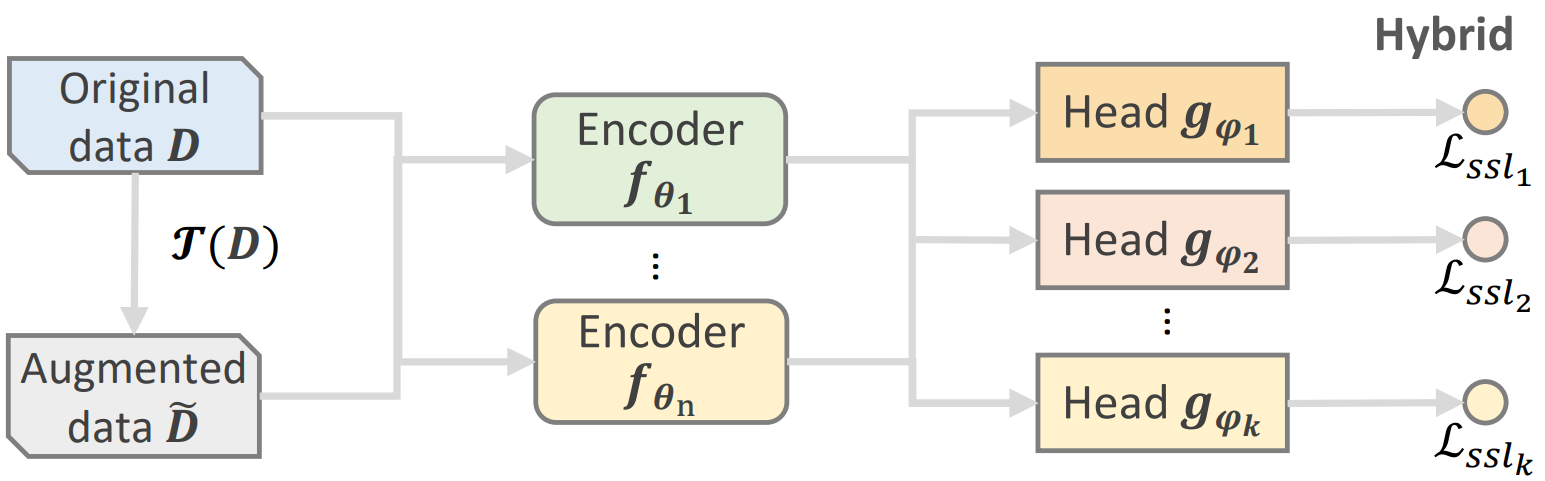
\includegraphics[scale=0.3]{images/Chapter3/hybrid_ssr.png}
        \captionof{figure}{Sơ đồ tổng thể phương pháp Hybrid trong bài toán Self-supervised Recommendation.}
    \end{minipage}
\end{itemize}

Trong phạm vi khóa luận này, ta sẽ tập trung giải thích việc áp dụng \textbf{Contrastive Learning} vào SSR và phân tích hiệu quả mà nó mang lại. Cụ thể hơn về việc áp dụng Contrastive Learning trong bài toán SSR như thế nào, ta mô tả chi tiết ở phần sau. Ngoài Contrastive learning, những phương pháp khác vẫn có rất nhiều tiềm năng phát triển và đáng được nghiên cứu trong tương lai, vậy nên ta chỉ mô tả ý tưởng chính chứ không tiếp tục đào sâu ở các phần sau.

\subsection{Kiến trúc tổng quát} \label{3.3.1-general-architecture}
% \subsubsection{Encoder}
% \subsubsection{Project head}
% Để cải thiện hệ thống gợi ý, kiến trúc của hệ thống sẽ bao gồm hai phần như trên hình. Phần thứ nhất, tác vụ gợi ý trên mạng học sâu đồ thị, đóng vai trò chính. Phần thứ hai, áp dụng contrastive learning với dữ liệu được tăng cường (dữ liệu này được tạo ra từ chính đồ thị gốc ban đầu, điều này sẽ giúp cải thiện việc học biểu diễn, từ đó bổ trợ, tối ưu cho cho tác vụ gợi ý.

\noindent Về mặt phương pháp áp dụng học tự giám sát, ta có hai thành phần chính. Phần thứ nhất đóng vai trò chính, học các biểu diễn cho node trong đồ thị và đưa ra dự đoán cho tác vụ gợi ý. Phần thứ hai áp dụng Học tương phản (Contrastive learning) với dữ liệu được tăng cường để cải thiện học biểu diễn, từ đó tối ưu cho tác vụ gợi ý.

\begin{figure}[H]
    \centering
    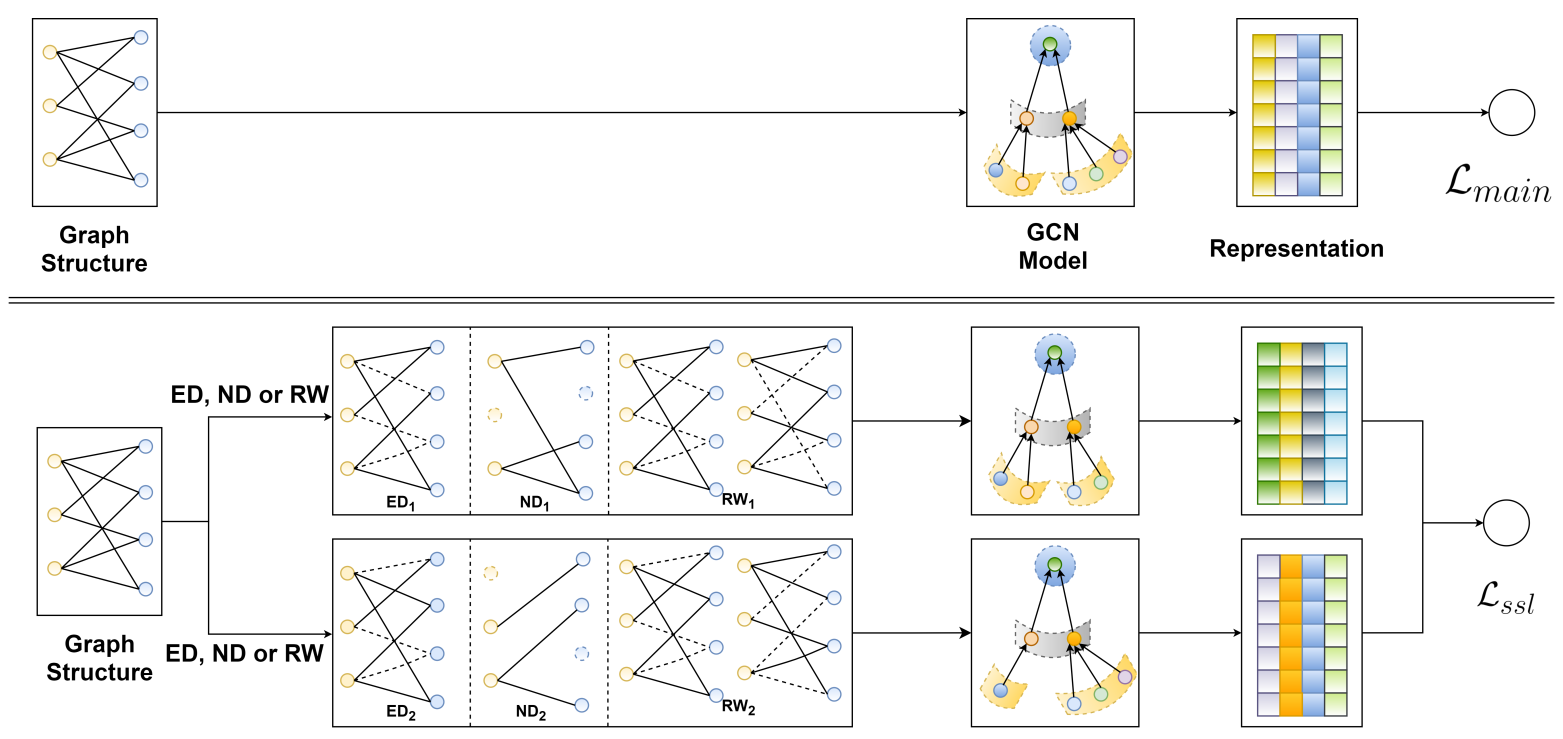
\includegraphics[scale=0.35]{images/Chapter3/sgl.png}
    \caption[Tác vụ chính và phụ của Contrastive learning.]{Trên: tác vụ chính (main task) cho gợi ý. Dưới: tác vụ phụ (pretext task) tối ưu học biểu diễn (Hình ảnh được trích từ bài báo của Wu \cite{SGL}).}
\end{figure}

Đối với việc tăng cường dữ liệu, hiện tại có rất nhiều cách tiếp cận, vì ma trận kề của đồ thị tương tác chính là ma trận đặc trưng của nó nên chỉ cần tập trung vào tăng cường cấu trúc đồ thị là đủ. Nói về đại ý, ta cần tạo các tăng cường dựa trên cấu trúc đồ thị gốc, làm thay đổi ma trận kề của đồ thị. Ta định nghĩa hai tăng cường của cùng một node sẽ được coi như là một positive pair và của các node khác nhau được coi như là negative pair. Nhiệm vụ tự giám sát phụ trợ sẽ thúc đẩy tính nhất quán giữa các positive pair, trong khi đó ép ra xa nhau đối với các negative pair trong không gian nhúng. Nhờ đó, ta có thể suy ra embedding một cách tốt hơn, từ việc quan sát và rút trích những đặc điểm, những cấu trúc bên dưới hoặc những khuôn mẫu đặc trưng nào đó của dữ liệu. 
% https://arxiv.org/pdf/2301.12189v1.pdf
% https://arxiv.org/pdf/2212.11491.pdf

\subsection{Áp dụng tăng cường dữ liệu}
\noindent Trong phạm vi khóa luận này, ta sẽ áp dụng các phương thức tăng cường \textbf{Edge dropout}, \textbf{Node dropout} và \textbf{Random walk} nhằm tạo ra các view khác nhau của node.

Về chi tiết mô tả tăng cường, ta đã đề cập ở phần \ref{3.1-data-aug}. Khi huấn luyện, ở mỗi epoch, ta sẽ tạo ra hai view cho mỗi node. Với hai phương pháp Edge Dropout và Node Dropout ta sẽ chọn lược bỏ một số cạnh/node với xác suất $\rho$. Hai view của các node trong Edge/Node dropout được chia sẻ và sử dụng chung trên các lớp trong mạng học sâu đồ thị. Riêng với Random Walk, ta sẽ chọn giữ toàn bộ node, với mỗi node, ta bước qua một vài node lân cận một cách ngẫu nhiên, với xác suất bỏ cạnh đi qua là $\rho$. Thêm nữa, để tăng tính ngẫu nhiên, tại mỗi lớp trong mạng học sâu đồ thị, ta sẽ tạo ra hai view khác nhau cho tăng cường Random walk.

Với ký hiệu như đã định nghĩa ở phần \ref{3.2.3-GNN-on-rec}, ta gọi embedding của hai view của cùng một node $v$ là $\mathbf{e}_v'$ và $\mathbf{e}_v''$.

\subsection{Học Tương Phản trên dữ liệu tăng cường}
\noindent Về mặt thống kê, các mô hình học máy được chia thành loại genrative và discriminative \cite{ssl-genorcont}. Hầu hết các nhiệm vụ học biểu diễn đều hy vọng sẽ mô hình hóa được các mối quan hệ giữa điểm dữ liệu đầu vào (input), vậy nên trong một thời gian dài, mọi người tin rằng mô hình Generative là lựa chọn duy nhất cho việc học biểu diễn.

Ở phần \ref{2.4-ssl}, ta biết rằng khi áp dụng Học tự giám sát, ta có rất nhiều cách tiếp cận khi mô hình học này lên mạng học sâu đồ thị. Ở phần \ref{3.2-graph-learning-recommender} ta cũng nhận ra để có được một biểu diễn của đồ thị đủ tốt và mang lại hiệu quả, các mô hình cần nắm bắt được các thông tin cần thiết từ cả thuộc tính nút và cấu trúc liên kết của đồ thị. Học tương phản nói riêng và mô hình discriminative nói chung đã mở ra một cánh cửa mới cho việc học biểu diễn như DeepInfoMax \cite{DeepInfoMax}, MoCo \cite{MoCo}, SimCLR \cite{SimCLR},... Hơn nữa, tính hiệu quả của nó cũng đã được chứng minh bởi Wu và các đồng nghiệp \cite{SGL}. Học tương phản sẽ được áp dụng như là một phương thức hay nói cách khác nó đóng vai trò không thể thiếu khi ta muốn áp dụng mô hình học tự giám sát trên mạng học sâu đồ thị nhằm làm tăng hiệu quả cho tác vụ gợi ý. Để áp dụng được phương pháp này, ta cũng cần một hàm mất mát phù hợp. Một loại hàm mất mát được áp dụng phổ biến và rất hiệu quả đối với học tự giám sát nói chung là InfoNCE \cite{InfoNCE, ssl-genorcont}, có dạng tổng quát như sau:
\begin{equation}
    \mathcal{L}_\textit{ssl} = \mathbb{E}_{z, z^+, z^-}\left[-\log{\frac{\exp(z^T z^+)}{\exp(z^T z^+) + \exp(z^T z^-)}}\right],
    \label{eq:general-NCE}
\end{equation}
với $\mathbb{E}[\cdot]$ là kì vọng, $\exp(\cdot)$ là hàm mũ cơ số $e$, $z$ là biểu diễn của một mẫu dữ liệu (tạm gọi là $x$), $z^+$ là biểu diễn của một mẫu dữ liệu mà giống với $x$, và $z^-$ là biểu diễn của một mẫu dữ liệu mà không giống với $x$. Khi cực tiểu hóa $\mathcal{L}_\textit{ssl}$, ta sẽ thúc đẩy tính nhất quán giữa $z$ và $z^+$, ép sự phân kì giữa $z$ và $z^-$. Nếu tập dữ liệu chứa nhiều mẫu dữ liệu không giống với $x$ thì công thức trên có dạng:
\begin{equation}
    \mathcal{L}_\textit{ssl} = \mathbb{E}_{z, z^+, z^k}\left[-\log{\frac{\exp(z^T z^+)}{\exp(z^T z^+) + \sum_{x^k \nsim x}{\exp(z^T z^k)}}}\right],
    \label{eq:more-dissim-NCE}
\end{equation}
với $x^k$ là những mẫu dữ liệu không giống với $x$. Để thực sự áp dụng công thức này vào học gợi ý, ta cần phải biến đổi đôi chỗ.

\subsubsection{Hàm mất mát InfoNCE}
\noindent Ở công thức \eqref{eq:general-NCE} và \eqref{eq:more-dissim-NCE}, ta nhắc đến mẫu dữ liệu với tính chất ``giống'' và ``không giống'' nhau, tức là trong tập dữ liệu, nếu xét về tính chất, đặc trưng,... thì hai mẫu dữ liệu đó có tập thuộc tính tương tự nhau, và ngược lại nếu như hai mẫu dữ liệu đó không giống nhau. Đối với bài toán gợi ý trên đồ thị thì như ta đã định nghĩa ở phần \ref{3.3.1-general-architecture}, cặp node positive pair sẽ được coi như là giống nhau, cặp negative pair được coi như là khác nhau. Với học gợi ý, Wu \cite{SGL} đề xuất một hàm mất mát phục vụ cho việc Học tương phản như sau trên ý tưởng của InfoNCE:
\begin{equation}
    \mathcal{L}_\textit{ssl}^\textit{user} = \sum_{u \in U}{-\log{\frac{\exp(s(\mathbf{e}_u', \mathbf{e}_u'') / \tau)}{\sum_{v \in U}{\exp(s(\mathbf{e}_u', \mathbf{e}_v'') / \tau)}}}},
\end{equation}
trong đó, $\tau$ là 1 hyper-parameter gọi là temperature trong softmax, $s(\cdot)$ đo sự tương đồng giữa 2 vector, dùng độ tương đồng cosine, công thức \eqref{eq:cosine-sim}. Ta có thể áp dụng công thức hàm mất mát trên tương tự cho sản phẩm. Từ đó, ta có hàm mất mát cho quá trình Học tương phản như sau:
\begin{equation}
    \mathcal{L}_\textit{ssl} = \mathcal{L}_\textit{ssl}^\textit{user} + \mathcal{L}_\textit{ssl}^\textit{item}.
\end{equation}

Wu và các đồng nghiệp \cite{SGL} phân tích hàm mất mát trên và đưa ra ưu điểm là nó giúp mô hình phân biệt các biểu diễn của những node khác nhau tốt hơn thông qua \textit{Hard negative mining}. Cụ thể là với những cặp negative pair mà có biểu diễn giống nhau, khó phân biệt, hàm mất mát sẽ có nhiều ảnh hưởng hơn so với những cặp negative pair dễ phân biệt được với nhau. Thông qua sự điều chỉnh phù hợp của tham số $\tau$, ta cũng sẽ điều chỉnh được độ nhạy của Hard negative mining.

Hàm mất mát trên có tính hiệu quả cao, tuy nhiên cũng không phải là không có bất cập. Ngoài InfoNCE ra, ta cũng sẽ thử nghiệm thêm với hai loại hàm mất mát khác nữa là \textbf{Decoupled} \cite{decoupled-loss} và \textbf{Debiased} \cite{debiased-loss}.

\subsubsection{Hàm mất mát Decoupled}

\noindent Theo Yeh và đồng nghiệp \cite{decoupled-loss} tìm hiểu được, hàm mất mát InfoNCE có chứa một hệ số negative-positive-coupling (NPC) giảm hiệu năng tự giám sát của model, đặc biệt là khi batch size nhỏ. Ngoài ra là trong InfoNCE, mô hình rất nhạy cảm với các hyperparameter, tức là các hyperparameter không tối ưu sẽ ảnh hưởng rất nhiều lên việc học tự giám sát một cách tiêu cực. Các tác giả của hàm mất mát Decoupled cho rằng với hàm mất mát của họ, mô hình sẽ tăng hiệu quả huấn luyện hơn mà không cần phải sử dụng batch size lớn. Không những vậy, khi batch size càng lớn thì mô hình càng học tốt hơn. Tổng quát của hàm mất mát này rất đơn giản: từ gốc là hàm mất mát InfoNCE, ta chỉ cần trừ hàm mũ $\exp(s(\mathbf{e}_u', \mathbf{e}_u'') / \tau)$ ra khỏi mẫu. Cụ thể, với các biểu diễn cho gợi ý, công thức hàm mất mát có dạng như sau:
\begin{equation}
    \begin{aligned}
        \mathcal{L}_\textit{decoupled ssl}^\textit{user} & = \sum_{u \in U}{-\log{\frac{\exp(s(\mathbf{e}_u', \mathbf{e}_u'') / \tau)}{\sum_{v \neq u}{\exp(s(\mathbf{e}_u', \mathbf{e}_v'') / \tau)}}}} \\
        & = \sum_{u \in U}{\left[-s(\mathbf{e}_u', \mathbf{e}_u'') / \tau + \log{\left(\sum_{v \neq u}{\exp(s(\mathbf{e}_u', \mathbf{e}_v'') / \tau)}\right)}\right]}.
    \end{aligned}
\end{equation}

\subsubsection{Hàm mất mát Debiased}

\noindent Chuang và đồng nghiệp \cite{debiased-loss} chỉ ra rằng, trong đa phần các model sử dụng Contrastive learning, với mỗi mẫu dữ liệu $x$, chỉ chọn ra một mẫu dữ liệu $x^+$ khác để kết hợp làm positive pair, ví dụ điển hình là mẫu dữ liệu này được trích ra từ bản sao tăng cường; nhưng song song với đó lại chọn nhiều mẫu dữ liệu $x^-$ khác để kết hợp làm negative pair. Bất cập của tiếp cận này là vẫn có khả năng là có một mẫu dữ liệu $x^-$ nào đó mà thực sự giống với $x$ nhưng lại bị thúc đẩy sự phân kì xét về mặt biểu diễn, ví dụ trường hợp hai người dùng khác nhau nhưng có chung tập sản phẩm đã tương tác. Hiện tượng này được Chuang và đồng nghiệp gọi là \textit{thành kiến trong việc lấy mẫu} -- \textit{sampling bias} mà có thể dẫn đến giảm hiệu năng trong thực tế.

Một hàm mất mát lí tưởng mà không có sampling bias trên thực tế không thể đạt được. Vì vậy, Chuang và đồng nghiệp xây dựng một tiếp cận mới để làm giảm tác động tiêu cực của nó -- Debiased. Ý tưởng chính là với tổng hàm mũ $\sum_{v \neq u}{\exp(s(\mathbf{e}_u', \mathbf{e}_v'') / \tau)}$ ở dưới mẫu, ta trừ đi một tỉ lệ của giá trị $\exp(s(\mathbf{e}_u', \mathbf{e}_u'') / \tau)$ để giảm đi tác động của việc phải phân kì các cặp $\mathbf{e}_u'$ và $\mathbf{e}_v''$ mà hai node $u$ và $v$ có thể giống nhau. Cụ thể, ta có phương trình tổng quát sau:
\begin{equation}
    \mathcal{L}_\textit{debiased ssl}^\textit{user} = \sum_{u \in U}{-\log{\frac{\exp(s(\mathbf{e}_u', \mathbf{e}_u'') / \tau)}{\exp(s(\mathbf{e}_u', \mathbf{e}_u'') / \tau) + \textit{Ng}}}},
\end{equation}
trong đó, $\textit{Ng}$ là hàm lấy giá trị lớn nhất $\max(\textit{Ng}', N \cdot \exp(-\frac{1}{t}))$ với $\textit{Ng}'$ là:
\begin{equation}
    \textit{Ng}' = \frac{-N \cdot \tau^+ \cdot \exp(s(\mathbf{e}_u', \mathbf{e}_u'') / \tau) + \sum_{v \neq u}{\exp(s(\mathbf{e}_u', \mathbf{e}_v'') / \tau)}}{1 - \tau^+},
\end{equation}
với $N$ là số lượng node $v \neq u$; $\tau^+$ là xác suất chọn một node $v \neq u$ nào đó mà thực sự giống với $u$, dùng để ước lượng mức độ ảnh hưởng của các cặp negative pair $(\mathbf{e}_u', \mathbf{e}_v'')$ thông qua cặp positive pair $(\mathbf{e}_u', \mathbf{e}_u'')$ khi giảm sampling bias trong tổng $\sum_{v \neq u}{\exp(\cdot)}$. Giá trị mẫu $1 - \tau^+$ dùng để bình thường hóa lại độ lớn của $\textit{Ng}'$ trong trường hợp giá trị trên tử quá nhỏ (gần bằng 0), tức là $\tau^+$ gần bằng 1. Việc tính $\tau^+$ cho mỗi node trong đồ thị là không thực tế, đặc biệt với lượng dữ liệu lớn, nên ta giả định $\tau^+$ đồng nhất với mọi node, và giá trị của nó là xác suất chọn một cặp negative pair bất kì trong toàn bộ tập dữ liệu mà lại thực sự giống nhau. Như vậy, tham số này có thể được ước tính từ tập dữ liệu hoặc là tự điều chỉnh (hyperparameter). Lấy $\max$ với $N \cdot \exp(-\frac{1}{t})$ chẳng qua là để tránh trường hợp lấy $\log$ của số âm; $t$ là hyperparameter khác.


\subsection{Phương án huấn luyện}
\noindent Trong thực tế, tác vụ gợi ý và pretext task (trong khóa luận này là Học tương phản) được kết hợp theo nhiều phương án (scheme) khác nhau tùy thuộc vào tình huống cụ thể. Ở trong phạm vi khóa luận này, ta sẽ sử dụng phương án \textbf{Joint Learning} \cite{survey:ssl-for-rec-sys} để giải quyết bài toán. 

\textbf{Joint Learning}: hiện nay, đa số các cách tiếp cận với học tự giám sát trên hệ thống gợi ý đều áp dụng scheme dạng này, đặc biệt là các phương thức contrastive. Lúc này, pretext task được bổ sung và cùng lúc được tối ưu với tác vụ chính là tác vụ gợi ý qua một encoder chung (ví dụ, trong khóa luận ta đang sử dụng một loại mạng học sâu đồ thị LightGCN). Kết quả tốt nhất ta có thể đạt được bằng cách điều chỉnh hyperparameter $\alpha$. Đây có thể được xem là một dạng multi-task learning.

\begin{figure}[H]
    \centering
    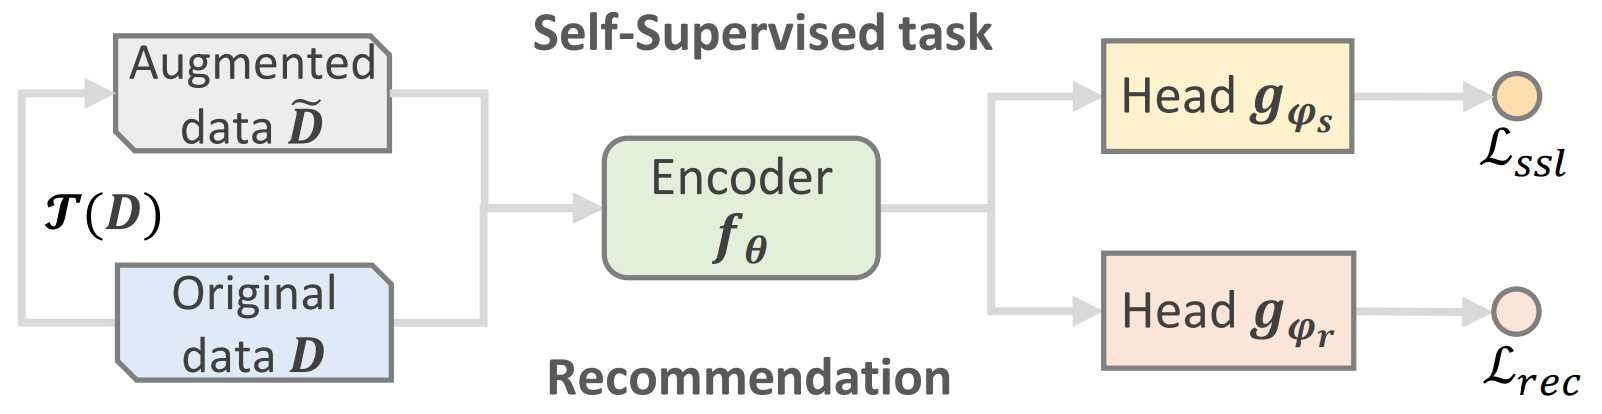
\includegraphics[scale=0.32]{images/Chapter3/jl_scheme.png}
    \caption{Sơ đồ Joint Learning.}
\end{figure}

\noindent Tổng quát hóa, ta giải bài toán tối ưu sau:
\begin{equation}
    f_\theta, g_\varphi, \mathbf{E} = \underset{f_\theta, g_\varphi}{arg min}\left[\mathcal{L}_\textit{rec}(g_{\varphi_r}(f_\theta(\mathcal{D}))) + \alpha \mathcal{L}_\textit{ssl}(g_{\varphi_s}(f_\theta(\tilde{\mathcal{D}})))\right],
\end{equation}
trong đó, hyperparameter $\alpha$ giúp điều chỉnh mức độ của tín hiệu học tự giám sát. Với công thức trên, ta sẽ sử dụng một hàm mất mát cho multi-task training đơn giản bằng cách kết hợp hai hàm mất mát của tác vụ gợi ý và tác vụ tự giám sát nhằm tối ưu cho hệ thống. Ta đi tìm cực tiểu cho hàm sau:
\begin{equation}
    \mathcal{L} = \mathcal{L}_\textit{rec} + \lambda_1 \mathcal{L}_\textit{ssl} + \lambda_2 \lVert \Theta \rVert_2^2,
\end{equation}
với $\Theta$ là tập hợp các tham số học của model; $\lambda_1$ và $\lambda_2$ lần lượt là các hyperparameter để kiểm soát mức độ ảnh hưởng của SSL và $L_2$ regularization, tương ứng. Với các kiến thức đã nói trước, ta có hàm mất mát sau cho mô hình học không giám sát trên đồ thị cho hệ thống gợi ý:
\begin{equation}
    \mathcal{L} = \mathcal{L}_\text{BPR} + \lambda_1 \mathcal{L}_\textit{ssl} + \lambda_2 \lVert \mathbf{E}^{(0)} \rVert_2^2,
\end{equation}
với $\mathcal{L}_\text{BPR}$ là hàm mất mát BPR \footnote{Trong hàm mất mát BPR cũng có regularization của tham số học của model. Ta sẽ kết hợp nó với regularization của Joint learning, và hàm mất mát BPR cũng sẽ được đơn giản hóa trở thành một hàm tổng $\ln(\cdot)$ duy nhất.}, $\mathcal{L}_\textit{ssl}$ là một trong ba hàm mất mát sử dụng việc học tương phản đã được định nghĩa ở phần trước, $\mathbf{E}^{(0)}$ là embedding của node (và cũng là tham số học) tại lớp thứ 0 của LightGCN. Tương tự như vậy, ta có Encoder $f_\theta$ là kiến trúc của LightGCN (công thức \ref{eq:lightgcn-encoder}).


% maximize mutual information như nào
% \begin{equation}
% L = E_{x,x^+,x^-} [-\log \frac{e^{f(x)} \cdot f(x^+)}{e^{f(x)} \cdot f(x^+) + e^{f(x)} \cdot f(x^-)}]
% \end{equation}

Ngoài Joint Learning (JL Scheme) ra, một số scheme khác có thể được áp dụng, tuy nhiên sẽ không được áp dụng trong phạm vi khóa luận này đó là \textbf{Pretraining and fine-tuning} (PF Scheme) và \textbf{Integrated Learning} (IL Scheme) \cite{survey:ssl-for-rec-sys}. Ta sẽ giới thiệu đôi nét về việc áp dụng hai phương án huấn luyện này và để dành việc khảo sát độ hiệu quả của hai phương án này cho các nghiên cứu trong tương lai.

\textbf{Pretraining and fine-tuning}: Phương án này cũng được sử dụng khá phổ biến. Đầu tiên, với pretext task, ta sẽ pretrain trên dữ liệu được tăng cường. Sau đó, ta sẽ sử dụng pretrain encoder thu được ở trên để fine-tune cho dữ liệu gốc. Cách này thường được dùng để huấn luyện các model SSR có dạng BERT, trong đó giai đoạn pretrain sẽ được áp dụng trên masked-based augmentation của input và sẽ được fine-tune trên dữ liệu chính. Ngoài ra còn được dùng khi pretext task để pre-train là contrastive method.
\begin{figure}[H]
    \centering
    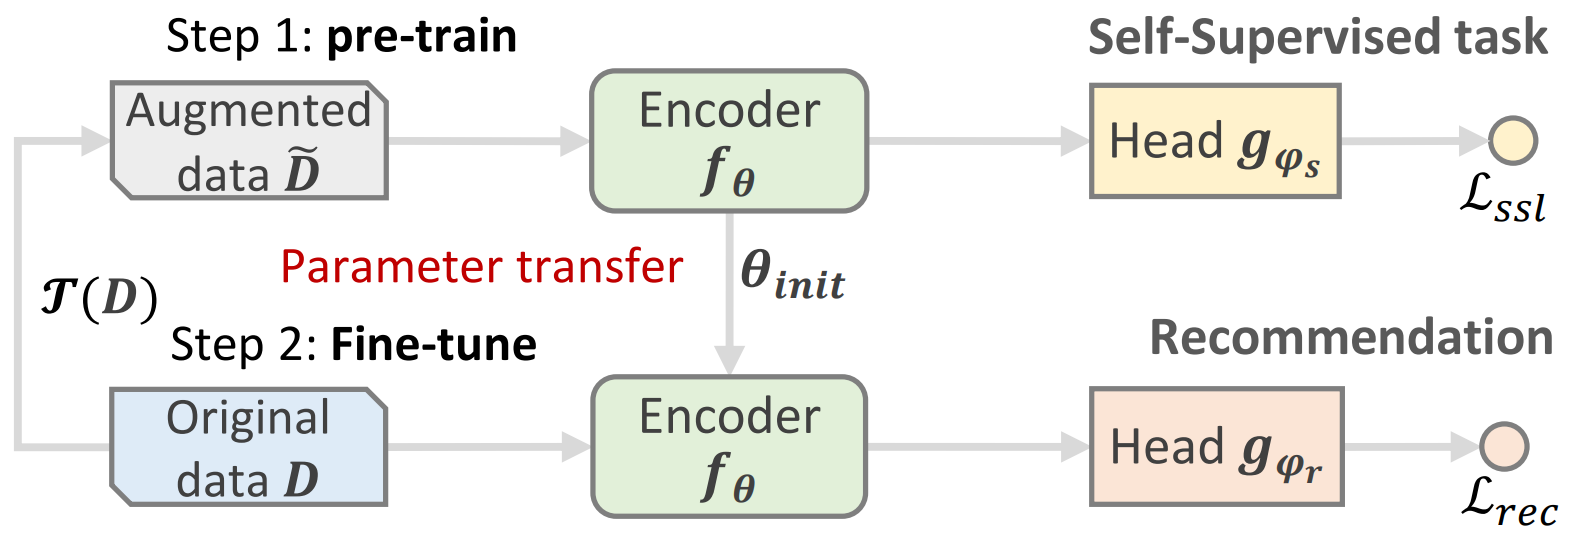
\includegraphics[scale=0.32]{images/Chapter3/pf_scheme.png}
    \caption{Sơ đồ Pretraining and fine-tuning}
\end{figure}

\textbf{Integrated Learning}: Khác với JL Scheme và PF Scheme, IL scheme thường được ít chú ý và biết đến. Lúc này pretext task và recommendation task được căn chỉnh sao cho output của cả hai là tương tự nhau.
\begin{figure}[H]
    \centering
    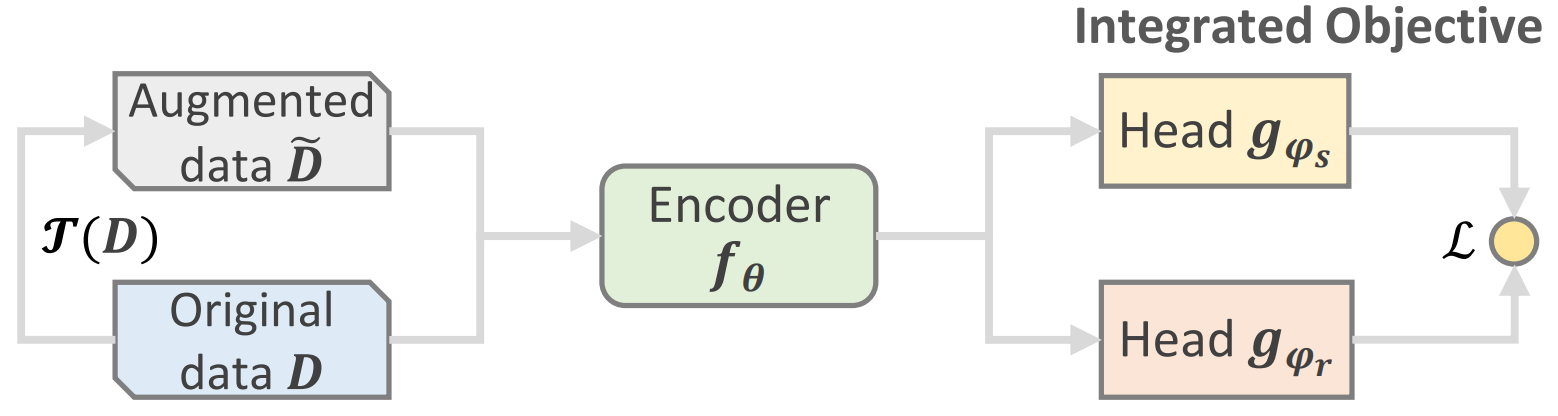
\includegraphics[scale=0.32]{images/Chapter3/il_scheme.png}
    \caption{Sơ đồ Integrated Learning}
\end{figure}

\subsection{Mã giả của thuật toán}
\noindent Sau đây là mô tả thuật toán tối ưu hóa các tham số của một model học tự giám sát trên đồ thị cho hệ thống gợi ý đã được mô tả ở trên. Ta có thuật toán SSL\_REC nhận đầu vào là các tham số $\mathbf{A}$ là ma trận kề của đồ thị tương tác, $\Theta$ là các tham số học ($\mathbf{E}^{(0)}$), cùng với đó là các tham số regularization $\lambda_1$ và $\lambda_2$. SSL\_REC sẽ đi tìm cực tiểu cho $\mathcal{L}$ bằng cách tìm giá trị cho $\mathbf{E}^{(0)}$ thông qua thuật toán Gradient descent với learning rate $\eta$. Ngoài ra ta định nghĩa đầu vào của các hàm sau:
\begin{itemize}
    \item[] \textbf{Encoder} $f_\theta(X, \mathbf{A})$: với $X$ là tham số của model, $\mathbf{A}$ là ma trận kề của đồ thị. Encoder trả về embedding cuối cùng $\mathbf{E}$ của model. Để ý là ta đang dùng kí hiệu $X$ thay vì $\mathbf{E}^{(0)}$ để dụng ý rằng $X$ là \textbf{biến} của hàm, trong khi $\mathbf{E}^{(0)}$ là một \textbf{giá trị} của $X$.

    \item[] \textbf{Hàm mất mát BPR} $\mathcal{L}_\text{BPR}(\mathbf{E})$: với $\mathbf{E}$ là embedding cuối cùng của model.

    \item[] \textbf{Hàm mất mát cho Học tương phản} $\mathcal{L}_\textit{ssl}(\mathbf{E}', \mathbf{E}'')$: với $\mathbf{E}'$ và $\mathbf{E}''$ là các embedding cuối cùng của hai đồ thị tăng cường được tạo ra. Để có được $\mathbf{E}'$ và $\mathbf{E}''$ thì ta chỉ cần lấy kết quả trả về của Encoder thông qua hai ma trận kề của các đồ thị tăng cường.
\end{itemize}
Ngoài ra ta cũng định nghĩa hàm $\mathcal{F}_\text{aug}(\mathbf{A})$ sẽ trả về ma trận kề của hai đồ thị tăng cường khác nhau từ ma trận kề gốc.

\clearpage
\noindent \textbf{Mã giả của thuật toán}
\begin{algorithm}[H]
    % \small
    \fontsize{14}{15}\selectfont
    \caption{SSL\_REC}
    \begin{algorithmic}[1]
        \Procedure{SSL\_REC}{$\mathbf{E}^{(0)}$, $\mathbf{A}$, $\lambda_1$, $\lambda_2$}
            \State initialize $\mathbf{E}^{(0)}$
            \Repeat
                \State $\mathbf{A}', \mathbf{A}'' \gets \mathcal{F}_\text{aug}(\mathbf{A})$
                
                \vspace*{+3mm}
                \State $\mathcal{L}(X) \gets \mathcal{L}_\text{BPR}\left[f_\theta(X, \mathbf{A})\right] + \lambda_1 \mathcal{L}_\textit{ssl}\left[f_\theta(X, \mathbf{A}'), f_\theta(X, \mathbf{A}'')\right] + \lambda_2 \lVert X \lVert_2^2$
                
                \vspace*{+3mm}
                \State $\nabla \mathcal{L}(\mathbf{E}^{(0)}) \gets \dfrac{\partial}{\partial X}\mathcal{L} \; \Bigr|_{\substack{X = \mathbf{E}^{(0)}}}$

                \vspace*{+3mm}
                \State $\mathbf{E}^{(0)} \gets \mathbf{E}^{(0)} - \eta \cdot \nabla \mathcal{L}(\mathbf{E}^{(0)})$
            \Until{convergence}
        \EndProcedure
    \end{algorithmic}
\end{algorithm}

% ssl method có thể đc áp dụng trên model graph bất kỳ
% 4. Phân tích SGL
